%
% Bachelor thesis of Eike Trumann
%
% Topic:
%

\documentclass[11pt,twoside,a4paper]{report}
%{{{ Packages

\usepackage[intl]{unibscnreport}
\usepackage[T1]{fontenc}
\usepackage[latin1]{inputenc}
\usepackage{graphicx}
\usepackage{makeidx}
\usepackage{multicol}
\usepackage{lgrind}
\usepackage{booktabs}

\def\pdfshellescape{1}
\usepackage{epstopdf}

%}}}
%{{{ Definitions

% Underline
\newcommand{\ul}[1]{\underline{#1}}
% Bold and sans serif
\newcommand{\sbf}[1]{\textsf{\textbf{#1}}}
% Raise box by half a line in tables
\newcommand{\rb}[1]{\raisebox{1.5ex}[-1.5ex]{#1}}
% Select language and switch off French spacing
\newcommand{\setlang}[1]{\selectlanguage{#1}\nonfrenchspacing}

% Search path
%\graphicspath{{abb/kap_tetra/}}

\pagestyle{headings}
\makeindex

%}}}

%\includeonly{introduced,conditions,sourcecode,citations}

\begin{document}

%{{{ Title page

\typ{Bachelor Thesis}
\title{Position-based Data Acquisition using Arduino and Android}
\author{Eike Trumann}
\betreuer{Dipl.-Ing. Jens Dede}
% In case that your supervisor has a master degree instead of
% a diploma, the degree is written after the name:
% \betreuer{K. Kuladinithi, M.Sc.}
\matnr{2840097}
\date{June 11th, 2017}
\makecntitle

%}}}
%{{{ Abstract, Kurzfassung

\cleardoublepage
\setlang{USenglish}
\thispagestyle{empty}

\begin{abstract}

  This thesis discusses the design of a system to acquire geotagged measure data. The system is based on the Arduino platform used to build a transducer device to which the sensors are connected and the Android platform which is used to run application software to visualize, store and export the data. On the Arduino platform, a software was developed allowing the integration of different sensors according to the needs of the user. The transducer device and the Android device running the application software use a Bluetooth communication channel to transfer the measured data. On the Android device, the application software can show the data received in a list and on a street map. The data can be written into a comma separated values file and exported to other apps or transferred to a personal computer.

\end{abstract}


\setlang{german}
\thispagestyle{empty}
\def\abstractname{Kurzfassung}

\begin{abstract}

  In dieser Abschlussarbeit wird der Entwurf eines Systems beschrieben, dass der georeferenzierten, also mit geografischen Koordinaten verbundenen, Messdatenerfassung dient. Als technologische Grundlagen werden hierbei die Arduino-Plattform als eingebettetes System, an dem Sensoren angeschlossen werden, und die Android-Plattform zur Darstellung, Speicherung und zum Export der Daten verwendet. F"ur die Arduino-Plattform wurde ein Software entwickelt, die eine Integration verschiedener Sensoren entsprechend des Bedarfes der aktuellen Anwendung erm"oglicht. Zur Kommunikation mit dem Android-Ger"at wird Bluetooth verwendet, wof"ur die Arduino-Hardware mit einem entsprechenden Modul verbunden werden muss. Auf dem Android-Ger\"at wird eine Applikation installiert, die alle vorgenannten Funktionen inklusive einer Visualisierung der Messdaten auf einer Stra\ss{}enkarte beeinhaltet. Die Daten k\"onnen aus der App in eine .csv-Datei exportiert werden, die mit anderen Apps ge\"offnet oder auf andere Ger\"ate \"ubertragen werden kann.

\end{abstract}

\setlang{USenglish}

%}}}
%{{{ Contents

\tableofcontents

%}}}
%{{{ Chapters

\chapter{Introduction}
\label{cha:Introduction}

Even though almost all sensors these days provide electrical or even digital data readout and data analysis tasks are carried out using a wide array of computer application software, there are still often analog gaps in the flow of information that need to be abridged by laborious human interaction. In an age of ubiquitous computing devices and network technologies researchers might still be found writing measured data on paper in order to transcribe it into a spreadsheet application later. The situation gets even worse if different types of sensors must be integrated or the measurements need to be conjoined with geolocation and time information.

Some of the reasons to persue a wasteful workflow abridging the analog gap might be the following:

\begin{itemize}
\item No suitable hardware has yet been build
\item High cost of avaliable systems
\item Existing systems are difficult to use
\item Lack of adaptability to use case
\end{itemize}

For this thesis, a measurement transducer that aims to overcome the aforementioned issues was build and tested. This thesis is mainly focused around so-called one-shot sensor readout (i.e. for each measurement there is only one value recorded for each sensor), but the system might easily be adapted for periodic sensor readout with frequencies up to around one sensor readout per second.

The system build for this thesis consists of a Google Android application and an embedded system build using the Arduino platform. The application might be installed on virtually any Android device. The basic functionality available includes receiving data from the Arduino part of the system using a Bluetooth connection and exporting the received information to a spreadsheet file that can be transferred to about any device or opened using third party application software on the Android device itself. The app can leverage Google's services to visualize data on a map and provide some other additional features.

The embedded system part basically consists of an Arduino (or compatible) microcontroller board and a Bluetooth transmission module. In case precise location information is needed, it is advisable to include a hardware GPS module (the geolocalization might also be handled by the Android device if it is eqipped with GPS). Any sensor that interfaces with Arduino (which includes sensors giving analog readout, UART serial connections, I$^2$C, SPI and more) might be included in the system. The information derived from the sensors is then sent to the Android application using a Bluetooth connection.

The rapidly increasing number of Android devices deployed, the widespread proficiency to use Android devices and low entry-level device prices are major strong points for the Android platform. Where available, pre-existing devices can be used in this setup without any further expenses for the Android part of system.

For the hardware parts of the system, the Arduino platform enables the hardware to be assembled by anyone with basic knowledge of electronic circuitry while the usage of the C-based Arduino programming language requires only little previous knowledge of embedded systems programming to adjust the code to new use cases.

\ section{State of the Art}
On the internet, a lot of Arduino projects including some sensors and communications to an iOS or Android smartphone can be found. Most of theese solutions are targeted at very specific purposes. Two projects that serve a purpose similar to the one of this thesis are Geo Data Logger (see \cite{gdl}), which is a software logging geotagged data from an Ardiono to a SD-card without any on-the-go visualisation capabilities and SensoDuino (see \cite{sensoduino}). While SensoDuino seems to offer most of the capabilities of the system described in this thesis including geotagged data logging, data visualization on Android smartphones and exporting the data to comma separated values files, the app is not avaliable as open source and seems to be abandoned not supporting recent Android versions. 

Commercialy available solutions (see \cite{mfEDV} and \cite{topcon} for examples of commercial products) often target only specific sectors like forestry, agriculture and construction works. None of these solutions offer the low cost and versatility of the system proposed in this thesis.


The system developed in this thesis aims to overcome the limitations imposed by the avaliable solutions and provide a versatile and low-cost alternative for both hobbyist and scientific use. An important aspect targeting these groups is the easy adaptability of the system eliminating the need to adapt the Android application software as many Arduino hobbyists and programming novices will find adapting Arduino software to be significantly easier compared to Android application programming.
\chapter{Requirement Specification}
\label{cha:requirements}
In this chapter, the basic requirements and properties for the parts of the system developed for this thesis are defined.

\section{Overall System Requirements}
The objective of this thesis is to develop and test a system to acquire position-based measurements. The resulting system should consist of two parts: An Arduino-based measurement transducer and a smartphone app.
The transducer should acquire the measurements from an arbitrary sensor (e.g., moisture, soil conductivity, soil stability etc.) when a button is pressed together with GPS-based position data. This data should be transmitted via Bluetooth to an Android smartphone. There, an app should receive this data, store and display it together with the position on a map. Additionally, the data should be exportable for example as a csv file.

In accordance with the supervisor it was decided that the system and the accompanying documentation should be published as open source software and thus the following objectives are especcially considered during the design phase:
\begin{itemize}
	\item Well-documented system design
	\item Code reusability
	\item Code comprehensibility
	\item Wide array of compatible hardware
	\item Hardware rebuildability even for inexperiences users
\end{itemize}

As it should be possible for interested inexperiences users to rebuild the system and adapt it to theier needs, clear entry points for modifications and a user-friendly documentation should be included.

\section{Hardware and Embedded Software Requirements}
From the basic goals of the system, some basic properties of the transducer hardware can be identified:
\begin{itemize}
	\item Battery powered
	\item Portable
	\item Based on the Arduino platform
	\item Broad range of compatible sensors
\end{itemize}

Furthermore there is a range of optmization criteria that may be derived from the task:
\begin{itemize}
	\item Energy consumption (battery lifetime)
	\item Compactness
	\item Low weight
	\item Sensor compatibility
	\item Extensibility
\end{itemize}

\subsection{Hardware}
It was decided the hardware should be based on the Arduino ecosystem as the Arduino system is a well-established and inexpensive hardware platform with low requirements for previous knowledge in embedded systems engineering. The ecosystem furthermore offers good documentation and a variety of software librarys for sensors and other external hardware.

It should be possible to build the hardware using inexpensive parts and having only basic knowledge of electronic circuits.

\subsection{Embedded Software}
The software should be able to run on as many device types of the Arduino platform as possible.

As it should be possible to use as many different sensor types as possible in the system, the code should be easily adaptable to support new sensors. Other than the hardware limitations, the number of sensors connectable should not be limited.


\section{Application Software Requirements}
The application software should run on as many different devices as possible including devices equipped with old Android versions and low-end hardware. Basic functionality (i.e. receiving data) must work without internet or other connections other than the Bluetooth connection to the hardware part of the system.

\subsection{Features}
The application must include means to receive, display, store and export the measurements.

\subsection{User Interface}
The user interface should be easy to use for new users and power users alike. 


%Survey of required components (GPS, Bluetooth) for Arduino
%Build the transducer (Hardware and Software)
%Implement communication between transducer and Smartphone (Bluetooth) Implement an Android Application to display, store and export the measurements
%Optimization of the overall system like
%Energy consumption of the transducer – PCB layout for the transducer
%Evaluation by performing outside field tests • Documentation and presentation of the work.
\chapter{System Specification}
\label{cha:system}

\section{Overall User Experience}
The user experience of the system must be considered for two different use cases. The first is a user receiving a pre-build and pre-programmed sensor transducer in order to perform measurements. The second is a user adapting the system to incorporate the sensors needed for his use case and assembling the required hardware.

\subsection{Measurement Workflow}
A user equipped with a pre-build device should be able to trigger a measurement with a single button push. 

Before being able to start the first measurement it is acceptable if the following steps are necessary:
\begin{itemize}
\item Connecting a power source to the transducer
\item Pairing the hardware module in Android Bluetooth settings
\item Starting the application software
\item Choose the hardware module in the application settings
\item Enable the connection in the application settings
\end{itemize}

The transducer device should then be ready to send data to the application software after a hardware button is pressed.

\subsection{Adaption to Use Case}
Adapting the system to a use case requiring specific sensors should be possible by performing the following steps:

\begin{itemize}
\item Finding a sensor model that can be interfaced with Arduino
\item Designing the appropriate electronic circuit to connect the sensor to an Arduino
\item Building the circuit
\item Extend the existing software to support the connected sensor
\item Deploy and test the embedded software
\end{itemize}

There should be no need to modify the Android application software as it should be designed to support arbitrary sensor types as long as the transmission protocol is respected.

\subsection{User Interface}
Apart from the button triggering a measurement, the user interface is a mostly a part of the application software. The application software should include at least the following features:

\begin{itemize}
	\item Visualisation of the measurement data as a list
	\item Visualisation of the locations where measurements have been made
	\item Recording of geolocation data (to be used if there is no discrete hardware GPS module or the module has failed)
	\item Exporting the data in a .csv file appropriate for different target applications like Microsoft Excel and Matlab
\end{itemize}

\subsubsection{Design Considerations}
The design of the application software should be clear and simple to use. Android users should not be surprised by unexpected application behavior. Where possible, native design elements and user interface paradigms should be used.

\section{Transmission Technology Selection}
Android devices generally offer a multitude of communication technologies which might be suited for communications between the transducer device and the Android application software.

\paragraph{Cellular Networks}
Cellular networks provide internet connectivity, voice and text message service covering wide areas. The spectrum used for these networks is normally regulated and can only be used having an appropriate contract with a network provider. This leads to higher operation cost when using cellular networks for communication purposes. The main advantage of using cellular networks would be the independence from the smartphone as data can be transmitted to the smartphone over long distances and buffered by the network or an internet service. While in Europe cellular network coverage is almost ubiquitous, in other parts of the world coverage might be spotty and using cellular network technology would impose additional data buffering needs on the system.

\paragraph{IEEE 802.11 (WLAN/WiFi)}
Wireless Local Area Networks (WLAN) are widely used for internet connections and general networking over medium (around 10 meters) distance. Using WLAN technology for a mobile use case has the major disadvantage of a device being only able to connect to one network at a time. This would mean the transducer must be either connected to the network that is used by the Android device for other communications as well (which might not even be possible for networks using complex authentication schemes like \emph{eduroam}). When used in a region without a known WLAN available, one of the devices would need to establish a network and make the other join it. 

\paragraph{Bluetooth}
The Bluetooth technology is used for so-called personal area networks. Bluetooth was originally designed to replace wired serial connections like the well-known RS232 standard. The Bluetooth technology till this day supports emulated serial ports which are transported over so-called RFCOMM-channels (see \cite{RFCOMM}). As all microcontrollers of the Arduino platform contain transceivers for serial communications (UART) at TTL voltage levels, they might easily interface with Bluetooth modules transmitting this serial data over an RFCOMM channel. Another advantage of the Bluetooth technology is the possibility to connect multiple devices at once. Bluetooth has a master-slave architecture where a master might normally connect to multiple devices at once, while a slave often can only connect to a single device. As the transducer does not need to connect to more than one device at once, the Android device might be configured as master and the Android device will still be able to connect to other Bluetooth devices simultaneously. There is a variant of the Bluetooth standard which is denoted Bluetooth Low Energy and used for low-bandwidth communications in newer devices.

\section{Communication Channel Specification}
\label{sec:protocol}
As interfacing the transmission technology to the microcontroller is easiest leveraging the Bluetooth technology and also other of the aforementioned arguments favor the use of Bluetooth as transmission technology, it was chosen as the carrier technology. Bluetooth supports different profiles targeted at different use cases. As commonly available Bluetooth modules for Arduino only support RFCOMM-channels and these channels do not need additional configuration, they are a reasonable choice as communication channels between the transducer and the Android device.

The communication used in the system is by nature heavily asymmetric regarding the data types transmitted and therefore the data protocol used by the serial communications over Bluetooth is also designed to be asymmetrical. 

\subsection{Android to Arduino}
In order to keep parsing mechanisms and transport code as compact as possible, a format using one character as the entire message is used. The transducer system does not need to implement this communication direction, however implementing it might significantly improve the overall user experience as it to some extent allows fault detection during use without controlling the correct data has been received on the Android device. The characters defined to be valid messages are the following:

\begin{description}
	\item [ACK] The ASCII acknowledgement character (0x06) is used to confirm measurement data was correctly received. If the transducer module would retransmit a lost message this symbolizes a retransmit is not necessary anymore. The transducer device may also contain a LED indicating an ongoing transmission until this message is received.
	\item [NAK] The corresponding NAK (Negative Acknowledge, 0x15) character should be sent if a parsing error occurs. If the transducer device is able to resend the measurement data this should trigger a resend.
	\item [DC1] The Device Control 1 character might be implemented to trigger a measurement the same way a button press on the transducer device does.
\end{description}

\subsection{Arduino to Android}
The main objectives for the data transmission format used from the Arduino to the Android devices are understandability and reimplementability.  Human-readability might be useful for debugging and testing purposes as it is much easier to hand-craft messages to include arbitrary contents and to recognize parsing errors when a human-readable format is used. The connection used for the communications between the Arduino and the Android devices allows for a fixed transmission speed to be used. As the penalty of waiting a fraction of a second longer for the data to appear on the Android device normally should be acceptable (especially if sensors producing long readout delays are included in the system), the compactness of the data representation is only a minor concern.

\subsubsection{Data Representation Format Selection}
\paragraph{JavaScript Object Notation (JSON)}
The JSON format (see \cite{ECMA-404}) is human readable and has has wide software support including the \texttt{org.json} library included the Android framework. As JSON allows for an object-oriented approach in data representation, the data con be converted (deserialized) into Java objects quite easily.

\paragraph{Extensible Markup Language (XML)}
XML (see \cite{XML}) is another text-based, human-readable data format widely used for various data storage and transmission purposes. On both the Arduino and Android platforms, libraries for XML encoding and parsing are readily available. XML is highly flexible in its use and allows the creation of schemas in order to allow formal validation, strong typing and other features. 

\paragraph{Concise Binary Object Representation (CBOR)}
CBOR (see \cite{CBOR}) is a binary (i.e. non-human-readable) data representation format putting the design focus on data compactness while using the same basic data model as JSON. While not included in the Android framework, there are usage ready libraries available for both Android and Arduino.

\paragraph{Custom Data Format}
In comparison to JSON and XML neither the understandability nor the reimplementability could be significantly improved by using a custom format. The effort needed for the implementation of a custom format is especcially high if high requirements for adaptability should be met.

\paragraph{Format Choice}
Based on the aforementioned data representation format choices the JSON format was chosen. Even though the serial communication is a low bandwidth connection (the maximum speed of typical Arduino Bluetooth modules is 115200 bit/s) the transmission time is not a critical piece of the overall system performance. As compactness would be the only advantage of CBOR, there is no reason to use CBOR in this application especially considering the obstacle a binary format imposes on embedded system debugging and testing.  A custom data format might be designed to be easy to debug but however would impose an unnecessary effort in data format compliance validation as well as format generating and parsing on anyone trying to reimplement parts of the system. This leaves the JSON and the XML formats as choices for the data transmission. Both formats provide about the same level of representation compactness, human-readability and ease of implementation. The additional features of XML do not provide a major advantage regarding embedded systems as including a full XML implementation would use more than the hardware resources available in typical embedded systems leading to the use of a stripped down version closely resembling the feature set of JSON.

Having the choice of JSON and XML left, the JSON format was chosen as it's object-oriented notation more closely resembles the data structures used in the Java programming language on the Android platform while providing a format that is easy to understand and modify for testing purposes.

\subsubsection{Data Format Specification}
As the data will be used in an Android application programmed in the object-oriented Java programming language, the data to be transmitted should be represented in an object-oriented way. While format-conforming data other then the specified might be included in the messages, this format specification provides the data fields that will be parsed correctly by the Android application software. In order to signal the end of the message an ASCII End of Text (0x03) character must be appended to the message.

In order to avoid problems in data transmission and representation any string in this transmission format must not contain special characters that could lead to JSON parsing errors (especially the ASCII End of Text character) or that could be understood as CSV separator characters (i.e. a comma, a semicolon or a tab stop).

\paragraph{General Information}
The general information data fields are placed in the root JSON object and provide information on the hardware and embedded software used. The name in parenthesis is the one specified to be included as key in the actual data transmission.

\subparagraph{Arduino Software Version (\texttt{arduino\_software})}
The Arduino software version is a string representing the software on the Arduino. 

\subparagraph{Arduino System Time (\texttt{arduino\_time})}
The Arduino system time is the time in milliseconds since the microcontroller was powered up or reset. This is a long integer and might later be used to understand Arduino system crashes (like power losses) and possibly detect unsolicited resends.

\subparagraph{Comment (\texttt{comment})}
The comment is a string that can (with the exception of special characters) contain arbitrary information the programmer of the sensor transducer embedded software might want to include. The comment might be later edited in the Android app to include additional information the system could not acquire automatically.
This string might be used to distinguish different measurement transducers (e.g. one transducer might include the comment \texttt{Temperature Transducer 1} and another \texttt{Humidity Transducer 2}).

\paragraph{Position  (\texttt{position})}
The position is a JSON Object including all relevant data that can be received using a GPS receiver. If the transducer hardware does not contain a GPS receiver, this object might be left out; if there is a GPS receiver, but there was no valid position fix yet or the position has not been updated for a significant time, the validity field should be set to \texttt{false}. If the validity field is set to false the rest of the data should be discarded and does not need to be transmitted. The position should be transmitted in geodetic coordinates as transmitted by GPS.

\subparagraph{Validity (\texttt{valid})}
This is a boolean field that should be set to true if there is a valid position included in the object.

\subparagraph{Age of the position fix (\texttt{age})}
The age field should include the integer number of milliseconds passed since the position transmitted was received.

\subparagraph{Latitude (\texttt{latitude})}
The latitude is a decimal floating-point number giving the geographical latitude in degrees (the decimal places are decimals of degrees and not minutes and seconds). The northern hemisphere is represented as positive numbers and the southern hemispheres as negative. Zero represents the equator. Any number outside the interval between -90 (south pole) and 90 (north pole) is invalid.

\subparagraph{Longitude (\texttt{longitude})}
The longitude is a decimal floating point number giving the geographical longitude in degrees (the decimal places are decimals of degrees and not minutes and seconds). The positive direction is defined as the eastern direction (seen from the prime meridian passing the Royal Observatory in Greenwich, London, United Kingdom). The valid range is from -180 to 180.

\subparagraph{Altitude (\texttt{altitude})}
The altitude in meters given by the GPS receiver represented as a floating point number. With concern to later data analysis it should be noted this is the height relative to the WGS84 ellipsoid. Altitude information derived from GPS data often has a relatively low accuracy.

\subparagraph{Calendar Date (\texttt{date})}
The date as transmitted by the GPS receiver (meaning based on the UTC time zone). The date must be represented as a decimal integer number in the ddMMyy (day-day-month-month-year-year) format. The system will need to be adjusted in case it should continue to run after the 21st century. 

\subparagraph{UTC Time (\texttt{time})}
The time given in the UTC time zone. The time must be represented as a decimal integer in the HHmmsscc (HH denotes a 24-hour format, mm is the minutes in an hour, ss the seconds in a minute and cc denotes metrical centiseconds) format. The time transmitted should represent the last GPS fix and not the time of the transmission. Note that GPS time is a time closely resembling UTC but not accounting for leap seconds. As of 2017 the GPS time differs from UTC by 18 seconds (GPS time in 2017 is UTC + 18 seconds).

\paragraph{Measured Data  (\texttt{sensors})}
The measured data is represented as a set of objects inside the sensors object (which is a child of the root object). Every object included in the sensors object must represent a single, real number measurement conforming to the data structure defined in this paragraph. This means sensors giving multiple outputs (e.g. a 3-axis accelerometer or a Hall effect sensor) must be represented as if they were multiple sensors. Sensors that do not have real numbers as output data are not supported. The objects representing the single measurement data can have an arbitrary name that might be used in debugging but is not part of the actual data that is received by the application software.

\subparagraph{Measured Property (\texttt{type})}
The measured property should be given as a descriptive string (preferably one word). The Android application software should translate this string when shown in the user interface if it is a common sensor type. If the measured property is in the list of the translatable types, the name should be given in the exact way mentioned in the appendix. If the measured value is not part of the list understood by the application software, this string is visible to the user. 

\subparagraph{Sensor type (\texttt{sensor})}
This should include an unambiguous type name for the sensor as a string.

\subparagraph{Name (\texttt{name})}
This should be a human-understandable form to know what property exactly is measured. This is especially useful if the transducer device includes multiple sensors recording the same measured property at different places. The name is arbitrary.

\subparagraph{Measured Value (\texttt{value})}
The measured value is represented as a real number. The unit is saved in a different field in order to allow easier ordering by value. The number must not be \texttt{NaN (Not a Number)} or infinity.

\subparagraph{Measurement Unit (\texttt{unit})}
The measurement unit represented as a string.

\paragraph{Data example}

\begin{verbatim}
	{
	  "position": {
	    "valid": true,
	    "age": 773,
	    "latitude": 53.10367584,
	    "longitude": 8.85041809,
	    "altitude": -4.60,
	    "date": 50417,
	    "time": 10543700
	  },
	  "sensors": {
	    "temperature-air": {
	      "type": "temperature",
	      "sensor": "DHT11",
	      "name": "air-temperature",
	      "value": 21.0000,
	      "unit": "deg C"
	    },
	    "humidity-air": {
	      "type": "humidity",
	      "sensor": "DHT11",
	      "name": "air-humidity",
	      "value": 28.0000,
	      "unit": "%"
	    },
	    "temperature-soil": {
	      "type": "temperature",
	      "sensor": "DS18B20",
	      "name": "soil-temperature",
	      "value": 22.75,
	      "unit": "deg C"
	    }
	  },
	  "arduino_software": "Arduino Pro Mini 0.2",
	  "arduino_time": 52142,
	  "comment": "Test Comment"
	}
\end{verbatim}

\section{Overall Data and Control Flow}
\label{sec:data_flow}
After the button triggering the measurement has been pressed, the Arduino microcontroller should collect the measure data from the attached sensors and transmit it to the Android Application. The basic process is shown in figure \ref{fig:data_flow}.

\begin{center}
\begin{figure}[h]
\centering
\makebox[\textwidth][c]{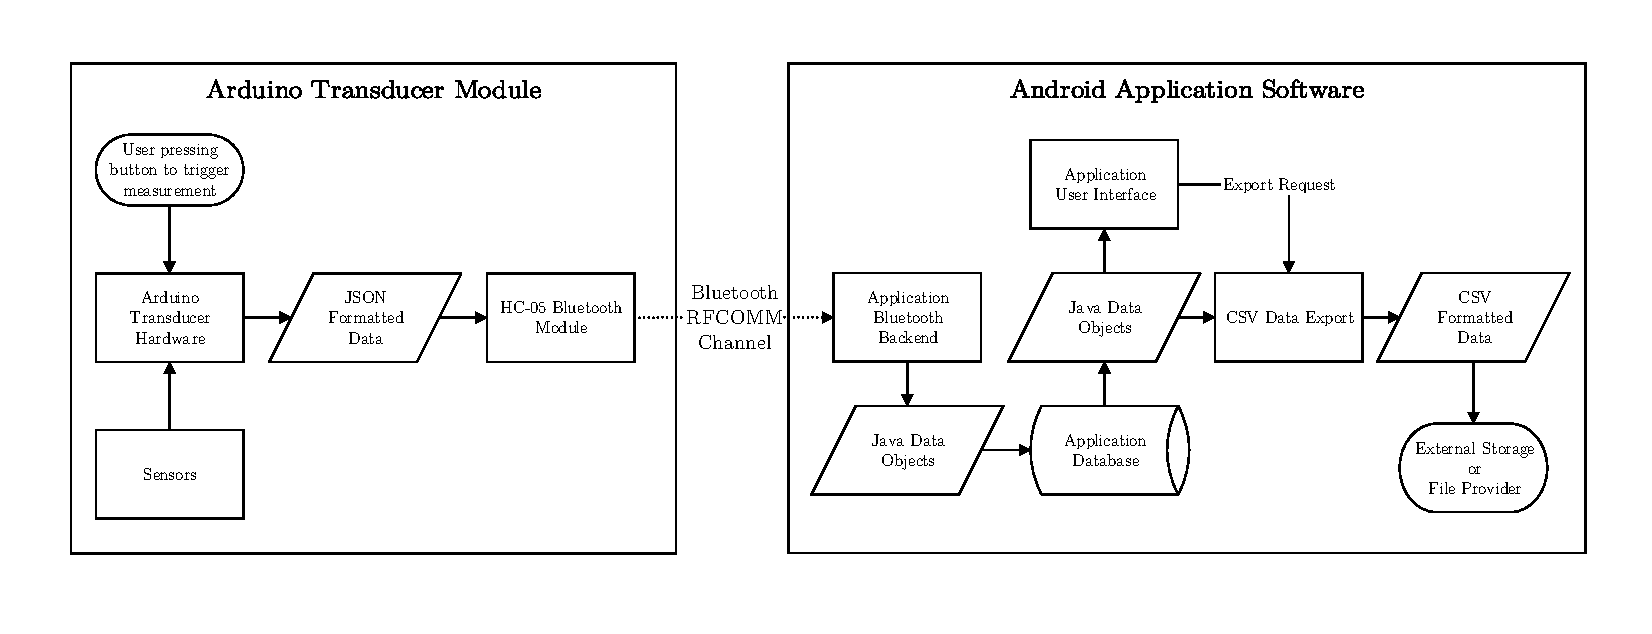
\includegraphics[width=1.1\textwidth]{src/data_flow.pdf}}
\caption{Data flow model for the overall system}
\label{fig:data_flow}
\end{figure}
\end{center}

\section{Positioning Strategies}
\label{sec:location}
Depending on the avaliable hardware and communications ressources the system shall be able to use different strategies to provide geolocalisation for the measured values. 

\subsection{Dedicated Hardware GPS Receiver}
A hardware GPS receiver can be incorporated in the sensor transducer hardware. It can operate independent of cellular network or WiFi data connections and can provide a better synchronization with the measurements triggered on the Arduino. Typically, GPS receivers are connected to the Arduino platform using a serial (TTL) connection transmitting so-called NMEA-sentences (see \cite{NMEASentences}) containing various values that can be derived from the GPS system including the location and the precise time. Dedicated hardware receivers usually allow for an external antenna to be connected which might give them a serious advantage in signal reception. The major downsides of a hardware receiver are the additional cost and the power consumption by both the GPS module and (if it is used) the external antenna.

\subsection{Android Device GPS}
Almost all Android smartphones and most Android tablets include a GPS receiver. However due to space constraints in the devices, the antennas in these devices are typically much less sensitive than dedicated external antennas. This often leads to poor GPS signal reception if the device is used in places having obstacles like trees, buildings and clouds in the signal path between the device and the GPS satellites. Compared to a hardware GPS receiver using the Android device GPS can have some advantages as most Android devices use assisted GPS to kickstart the GPS receiver with information derived from cellular and WiFi networks and some newer devices additionally include receivers for the GLONASS, BeiDou and Galileo global navigation satellite systems (GNSS).

\subsection{Googles Fused Location Provider}
The Fused Location Provider is a high-level API for localization services provided by the Google Play Services, a software library available on most Android devices (all devices using Google Play Store). The Fused Location Provider aggregates information derived from different sensors of the device and from an online service (which for example maps WiFi networks to location). The Fused Location Provider should always give results of the same or better quality compared to the device GPS at the same or a lower power consumption.

\subsection{Synchronization}
As the system might be moved during use, it is important to get not only accurate location information, but also location information synchronized to the measurements. A hardware GPS receiver does usually provide a new location in a regular interval like 1 second. This means as long as the position fix is not lost, the hardware GPS might always provide a location not older than one second. Both aforementioned Location Providers on the Android device are able to deliver location information at regular intervals too. However, using the aforementioned Location Providers in Android will lead to high energy consumption when periodic location updates are requested. As the Location Providers might also be used to provide a one-shot position fix, energy can be saved by requesting the location only in case a measured value has been received. The risk associated with this is a position drift caused by moving the device during the positioning delay. While the GPS provider can either deliver a position fix or not, the Fused Location Provider can be configured to give a high accuracy result as fast as available or give a lower accuracy result after a specified time in case a high accuracy fix is not possible. This makes the Fused Location Provider the preferred choice for one-shot location fixes.

\subsection{Performance Comparison}
With the Android platform having a huge number of different devices available, a comprehensive positioning performance test can not be undertaken in the context of this thesis. To verify the usefulness of a dedicated hardware GPS receiver however a spot test was carried out to compare the performance of some exemplary devices. The devices included in the test were the following:

\paragraph{Adafruit Ultimate GPS Breakout v3 and external Antenna}
This is a widespread dedicated hardware GPS module (see \cite{AdaGPS} for the Arduino platform. The GPS module was connected to an external antenna (see \cite{ExtAnt}) offering 28 dB of gain. The GPS module itself has a sensitivity of -165 dBm. The GPS module was equipped with a buffer battery allowing it to fix the position faster as previous knowledge of the time can be used (the module contains a real-time clock).

\paragraph{Nexus 7 (2012)}
The Nexus 7 (2012) (see \cite{Nexus7}) is a widespread Android tablet released in 2012. It does not offer a cellular data connection. For the performance comparison test, this device was set to flight mode and no data connection was available during the positioning. The data used in this test was derived using the Fused Location Provider (set to high accuracy) in one-shot mode; there was no active background GPS. The operating system used was the Android-based Resurrection Remix OS (see \cite{ResurOS}) equipped with Google Apps and the Google Play Services.

\paragraph{Ulefone Power}
The Ulefone Power (see \cite{UlePow}) is a smartphone running Android 6.0 Marshmallow. For this test, the Fused Location Provider (set to high accuracy) was used in one-shot-mode while the GPS provider was kept active in the background. An LTE cellular network connection was active at all times.

\subsubsection{Test Setup}
The test was carried out by moving the devices repeatedly between two fixed positions around 200 meters apart. The position was then recorded while all devices were at rest and at most 20 centimeters apart. Both locations have unobstructed view to the sky and the test was carried out under clear blue sky without any clouds.

\subsubsection{Test Result}
The test data has been imported into the Matlab software (see \cite{MATLAB}) and plotted to a web map. This map is shown in figure \ref{fig:gps_comparison}. While no statistical tests were carried out, performance differences can visually be deducted from the map. The raw measurement data and the script used to plot the map are included in the digital appendix.

\begin{figure*}[t]
\centering
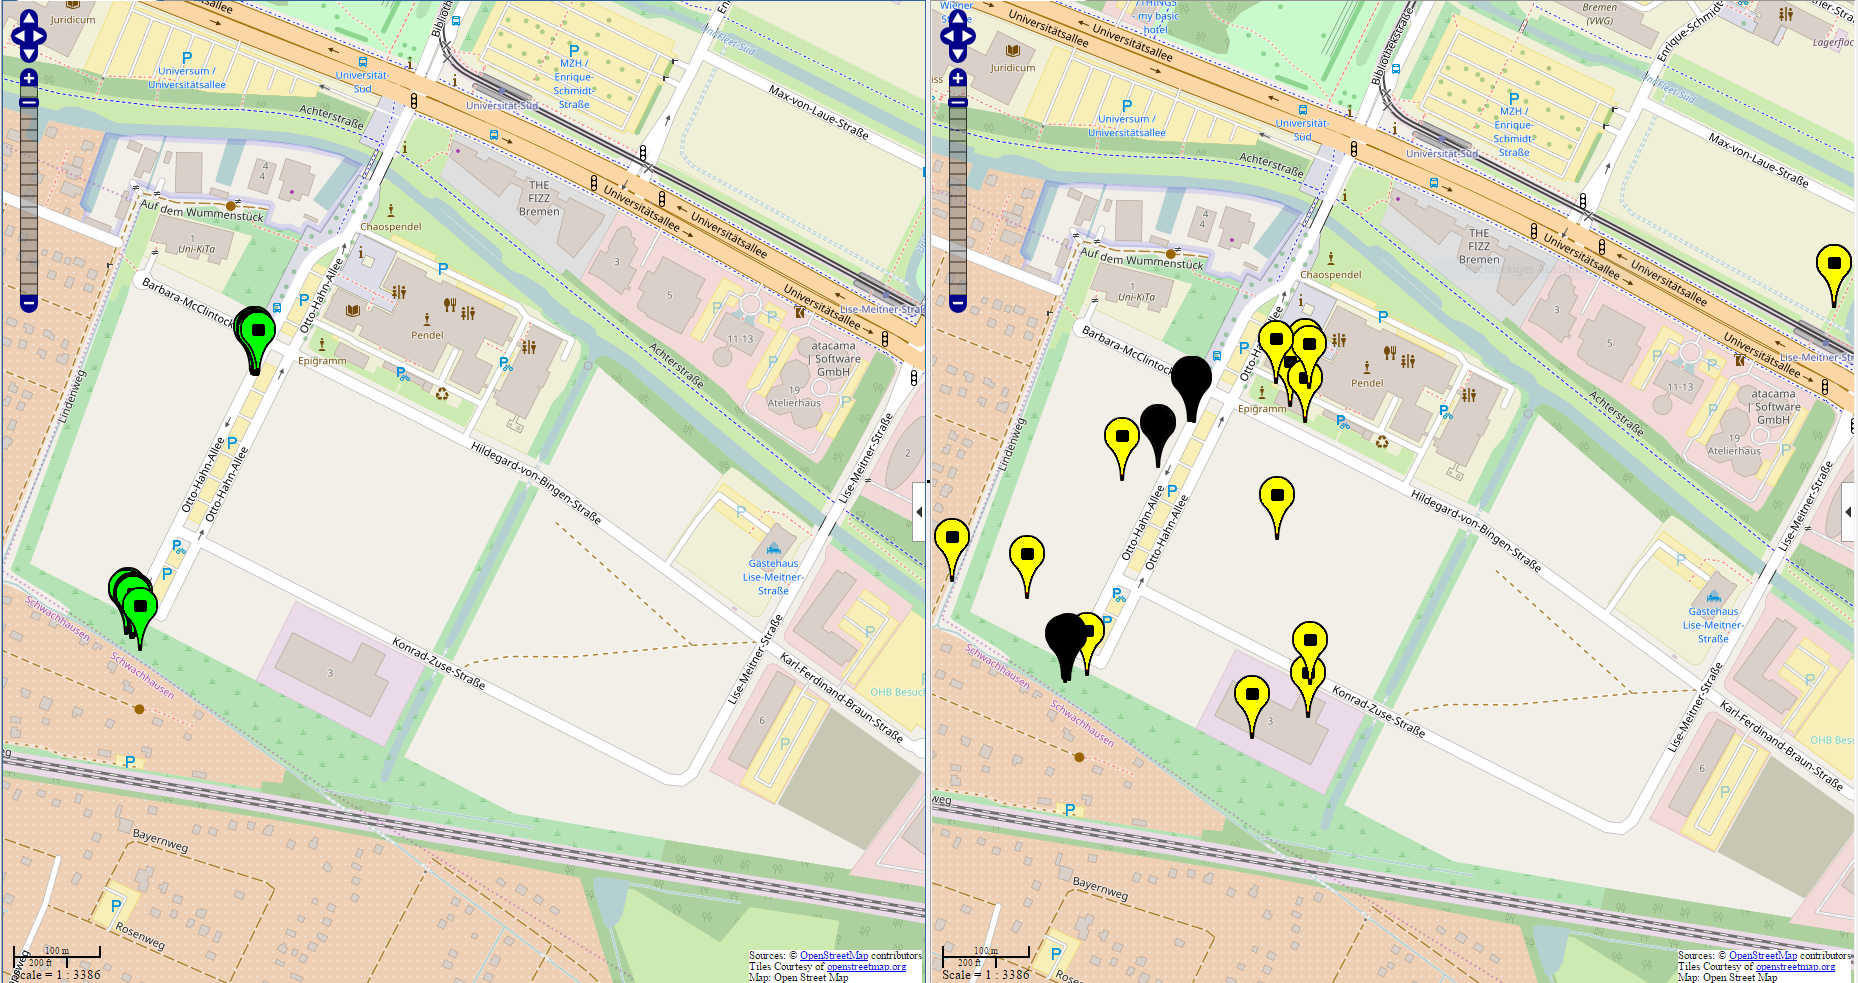
\includegraphics[width=1.0\textwidth]{src/gps_comparison.png}
\caption{Visualisation of the positioning test results. Left: Adafruit Ultimate GPS v3, Right: Black markers for the Nexus 7 and yellow markers for the Ulefone Power}
\label{fig:gps_comparison}
\end{figure*}

\subsubsection{Conclusion}
As seen on the map in figure \ref{fig:gps_comparison}, results derived from the Adafruit GPS module do vary only slightly between the measurements. The markers are covering the actual position of the measurements and do not differ by more than 10 meters from the actual position. The Nexus 7 (the black markers in the right map) exposes a similar result with one marker being on the way between the positions where the measurements have been triggered. The deviating marker marks the first measurement and is a result of movement during the positioning delay which could have been avoided if background gps positioning was enabled before this test. 

The Ulefone Power, even though its technical means to acquire a position seem much better as cellular networks and WiFi positioning were available as well, shows significant and obvious scattering of the location data acquired. The Fused Location Provider in this case reports a widely varying accuracy, but even when the reported accuracy is accounted for, the overall performance must still be considered poor compared to the other two devices.

In conclusion no general statement can be made on the positioning accuracy provided by Android devices. As a design decision, the system should therefore allow both dedicated hardware GPS receivers and the capabilities of the Android device to be used.

\subsection{Implemented Positioning Strategies}
The preferred approach is incorporating a GPS receiver in the sensor transducer hardware, however the Android app should contain means to record the location from the Android device's means of localization. 
\chapter{Hardware and Embedded Software}
\label{cha:hardware}

\section{User Interface}
As most of the user interface capabilities should be included in the Android application software, the transducer hardware can be designed to include only very basic user interface elements.

\paragraph{Input}
As the system should include the possibility to trigger measurements pushing a hardware button on the transducer device (rather than unlocking the Android device, starting the app and triggering the measurement there), a single button is needed which needs to be wired to an Arduino input able to trigger an interrupt. The pin is configured as as an input with the pull-up resistor enabled. The button connects the pin to ground while it is pushed; an interrupt accordingly is triggered on a falling edge of the pin input signal.

\paragraph{Signaling}
In order to let the user know if the device is ready for operation, it includes three LEDs that show the status of different system components:

\paragraph{Sending Indicator}
This LED has two use cases. It should light up when the user triggers a measurement and turn off when the Android device acknowledged having received the data. This means it gives a fast response to users showing their button press was received and it signals the time needed to handle the button press. The time needed to collect the sensor data might be significant and thus the user is informed that he should not trigger another measurement while the previous one is not completed. If the LED does not turn off, it indicates a connection fault and the user might need to address this by connecting the Android devece.

\paragraph{Bluetooth Status}
The bluetooth status LED should show the connection state of the bluetooth module. As most bluetooth modules do not directly transmit the connection state to the Arduino, the LED should be connected directly to the bluetooth module and relay the signalling normally shown by the internal status LED. Most modules contain a state pin to get this signal. If there is no possibility to get this signal, the LED might be left out.

\paragraph{GPS Status}
The GPS status can be derived either from the GPS module directly or queried in the embedded software. As the embedded software is closer to the transducer output, the state is determined in the embedded software and thus the LED is connected to an Arduino output pin (note that some Arduinos including the Arduino Due can only drive small currents and an appropriate current limiting resistor must be used).

\section{Hardware Requirements}
In general, it should be possible to build the sensor transducer hardware based on any Arduino. The setup must include a Bluetooth serial pass-through module. 

\section{Hardware Selection}
As the complexity of the project might significantly increase when a multitude of different hardware components must be supported, this section defines the requirements applied to the hardware and proposes suitable common components which are also used for the demonstration assembly.

\subsection{Bluetooth Module}
As defined in the previous chapter, the communication between the transducer hardware and the Android device should use the Bluetooth radio frequency communication (RFCOMM) profile. Any module that is able to pass serial data received via a TTL connection through to a Bluetooth RFCOMM channel should work for this purpose. In order to avoid damages to the hardware, the module either needs to use the same voltage as the Arduino or voltage limiting circuitry needs to be included. 

The proposed module is the HC-05 on a ZS-040 (see \cite{HC-05}) carrier board. This combination is commonly available and can typically be manually reprogrammed using AT-commands. Most of the carrier boards include a state pin which can be connected to the status LED. The only alternative commonly found is the HC-06 module which for this use case does exactly the same as the HC-05 module (while it does not support working as a Bluetooth master).

\subsection{GPS module}
As most GPS modules commonly available for discrete electronic circuits are using standardized NMEA-sentences to transmit the received data, these modules can be used interchangeably. The embedded software designed for this project exclusively supports GPS-receivers transmitting their data encoded as NMEA-Sentences via a serial (TTL) connection.

The module used in the demonstration device is an Adafruit Ultimate GPS (see \cite{AdaUltGPS}) module as it provides some useful additional features by allowing an external antenna to be connected via a $\mu$FL-connector and including an enable pin which can be used to disable the module. 

\section{Sensor Hardware Compatibility}
The Arduino platform is well known for its wide sensor compatibility. Typically, a library providing some kind of abstraction from the actual sensor interface is used and can easily be deployed to adapt the code for new sensors. 

Most Arduino boards provide the following interfaces for sensors:
\begin{itemize}
	\item UART (serial communications)
	\item I$^2$C (Inter Integrated Circuit, also called Two Wire Interface or TWI)
	\item Analog voltage input (10 or 12-bit resolution)
	\item Digital IO (used e.g. for the one-wire-bus)
	\item SPI (Serial Peripheral Interface Bus)
\end{itemize}

All of these interfaces can be used to connect sensors and other data sources. The software system is intended to be used with sensors that produce real (i.e. floating point) numbers as measurement output. The main design goal is support for one-shot readout, but sensors regularly producing data and sending it to the Arduino might as well be used.

Some Arduino models support additional interfaces such as CAN (Controller Area Network), Bluetooth, Sigfox (a low-power, long range wireless network technology) or GSM (standard cellular networks). These interfaces might be used according to their availability on the hardware platform chosen. 

If a sensor not directly compatible with the chosen hardware platform should be used, often converter modules can be used to transduce the data to a compatible interface. Common examples are high-resolution analog-digital converters connected to the I$^2$C-bus or CAN-Modules connected to the Arduino SPI bus.

\section{Circuit Wiring}
\subsection{Power Supply}
As the module should be usable everywhere, it cannot rely on mains power and therefore needs an independent power source. While powering the module from the Android device might be an option on some Android devices (which support on-the-go power via USB and contain an appropriate voltage regulator), doing so would neither be possible in general nor practical as it would quickly discharge the device battery. Therefore an independent battery should be used. All Arduino boards contain linear voltage regulators that can be used to regulate feed voltages that typically need to be around 0.3 Volt above the required device voltage. A 3.3 V Arduino can therefore be operated from any voltage above 3.6 V DC and a 5 V model typically needs 5.3 V (6 V is recommended) to be fed to the linear regulator. On 3.3 V boards this allows the system to be operated from a single LiIon-Cell or at least three NiMH or Alkaline batteries. As Lithium Batteries require extra components to be charged and to prevent deep discharges or short-circuits, the proposed device should be operated from NiMH rechargeable or alkaline primary battery cells. These cells can be exchanged by the user and in case of NiMH rechargable cells be recharged using standard chargers. Using alkaline primary batteries allows the device to be used with widely available batteries bought from a store in case no charging facilities are avaliable. The recommended size is AA (mignon), as this size provides a reasonable runtime for the device. Even though using only three cells might provide a sufficient voltage, using four cells is recommended for 3.3 V devices as the cells voltage will drop during discharge and on energy usage peaks. Using four cells allows the cells to be discharged to a typical end-point voltage of 0.9 V per cell instead of 1.2 V if only three cells are used.

\subsection{General considerations}
As the device should be as easy as possible to build, it should be possible to build the transducer module without soldering. As many sensors are available as modules that can be plugged into a breadboard or connected using jumper cables, it is recommended to use this kind of sensors. The wiring can then be made on a breadboard and using jumper wires which in turn makes the assembly modifiable and the modules reusable for other purposes when the transducer is not needed anymore.

Using a 3.3 V Arduino Pro Mini as an example, the basic circuit wiring is shown in figure \ref{fig:pro-mini-diagram} and a visual representation of the assembly on a breadboard is shown in figure \ref{fig:pro-mini-diagram}. Using other Arduino modules typically requires the Arduino to not be directly plugged into the breadboard but connected using jumper wires instead.

\begin{figure*}[t]
\centering
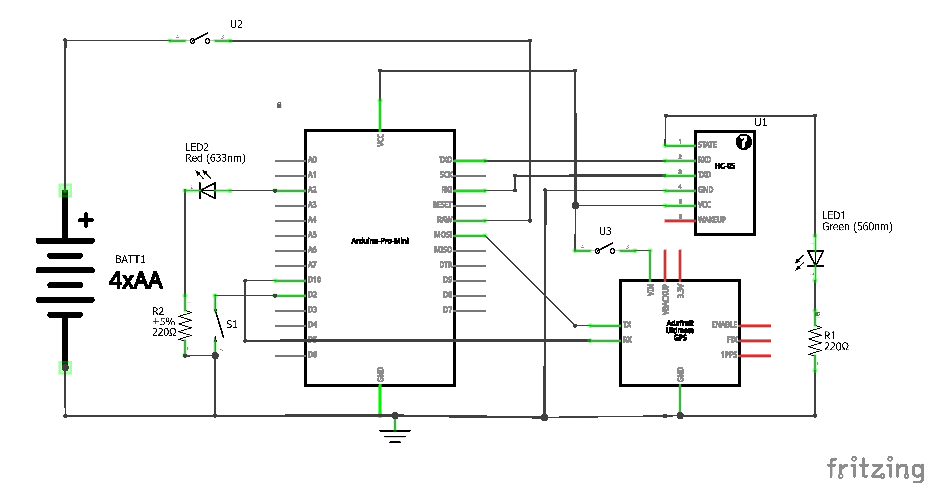
\includegraphics[width=1.0\textwidth]{src/pro_mini_diagram.pdf}
\caption{Proposed circuit for the basic transducer parts}
\label{fig:pro-mini-diagram}
\end{figure*}

\begin{figure*}[t]
\centering
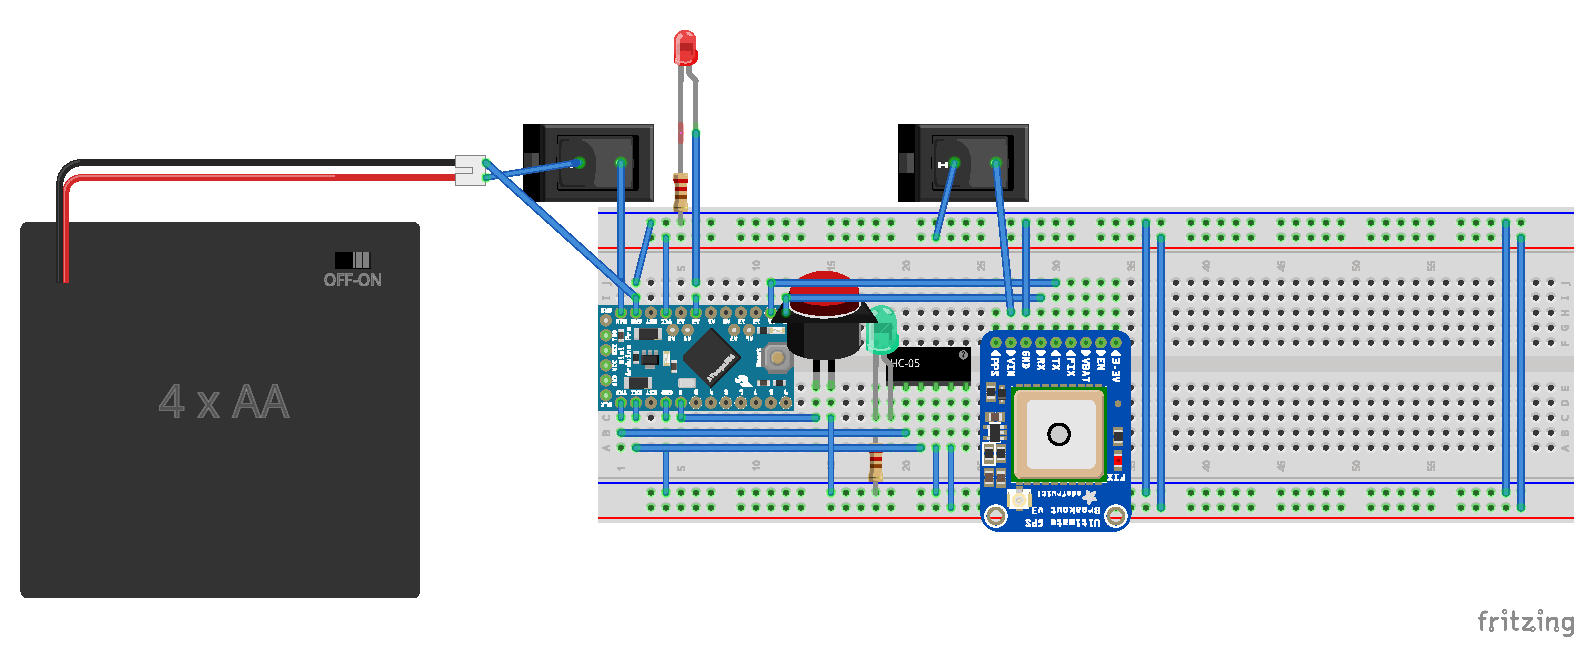
\includegraphics[width=1.0\textwidth]{src/pro_mini_breadboard.pdf}
\caption{Breadboard wiring example for the basic transducer parts}
\label{fig:pro-mini-breadboard}
\end{figure*}

\subsection{Demonstration Assembly}
The demonstration assembly is the version of the transducer device used for performance and energy-usage testing. It uses a 3.3 V Arduino Pro Mini module, the HC-05 Bluetooth Module and an Adafruit Ultimate GPS Module connected to an active external antenna. The power is supplied by four AA-size NiMH rechargeable batteries. The assembly follows the circuit wiring proposed in the previous section.

In order to test the system using actual sensors, a DHT11 air humidity and temperature sensor and an encapsulated DS18B20 digital temperature sensor are connected to the Arduino module. This sensors have a low energy consumption and will be included in all system performance tests.

\subsection{Case}
As the electronic components need to be protected from mechanical forces and accidental short circuits, a case for the demonstration assembly has been made using a 3D printer. The case was designed using Autodesk Fusion 360 (see \cite{f360}). The case was specifically designed to include the user interface elements used in the demonstration assembly. Design files for the base element and the top part can are included in the appendix. 

\begin{figure*}[h]
\centering
\includegraphics[width=1.0\textwidth]{src/demonstration_device.jpg}
\caption{The demonstration device enclosed in its case. On the left side, the cable connecting the external temperature sensor exits the case.}
\label{fig:demonstration_device}
\end{figure*}

\section{Energy Consumption Optimization}
As the system should be able to run on battery power, a long runtime before the batteries need to be changed is desirable. Therefore, the following proposed optimizations have been reviewed.

\subsection{Bluetooth Low-Energy}
The Bluetooth low energy standard was designed to allow significantly reduced energy consumption when compared to classic Bluetooth. As manufacturers of electronic modules for Arduino often do not publish information on energy consumption of their modules, the effects need to be measured in real testing devices. A Hameg Instruments HM8134 laboratory power supply has been used to measure the power consumption of the HC-05 Bluetooth module proposed for the transducer and a pin-compatible HM-10 Bluetooth low energy module. Both modules are specified to be used with a 3.3 V (dc) 50 mA power supply. The modules contain a low-dropout voltage regulator and can therefore be fed using higher voltages, however in this experiment, both modules are fed using 3.3 V and stabilized using a 1000 $\mu F$ capacitor next to the power input pins of the modules.

The modules differ significantly in their energy usage patterns. The HM-10 Bluetooth low energy module has a virtually constant current draw of around 9 mA. Opposed to that, the HC-05 module uses different currents depending on the connection state. While the module is searching, the current draw is around 40 mA, when connected and idle the module draws between 2 and 4 mA. When a message is sent, the current peaks to about 20 mA and stays around 15 mA for about 5 seconds. As the connection should be in the connected idle state for most of the time, the energy usage using the HC-05 Bluetooth module is significantly lower than using the HM-10 Bluetooth low energy module in most use cases. Therefore, it was decided to not include the option to use this Bluetooth low energy module in the system.

The average current values when run at 3.3 V supply voltage recorded during the measurements are the following:
\begin{center}
  \begin{tabular}{ | c | c |}
    \hline
	\hline
    HC-05 Bluetooth module (connected) & 2.38 mA \\ \hline
    HC-05 Bluetooth module (searching) & 39.91 mA \\ \hline
    HM-10 Bluetooth LE module (connected) & 10 mA \\ \hline
    HM-10 Bluetooth LE module (searching) & 8.88 mA \\ \hline
    \hline
  \end{tabular}
\end{center}

\subsection{Interrupt-Driven Programming}
Microprocessors typically include means to enter power saving states while only a limited subset of the processors capabilities are needed. While a microprocessor is waiting for user input it can often be put into a sleep state that includes the capability to wake up the processor when an external interrupt occurs. However, the Arduino software platform proposes the use of so-called busy loops to implement software features. As the energy usage of the complete Arduino module can be measured to be 5 mA using the same method as for the Bluetooth modules, the cost of breaking the Arduino programming paradigm in order to reduce the energy usage is considered unreasonable. Furthermore, the way GPS data is received on devices having only a single hardware serial transceiver imposes further problems when an interrupt driven programming model should be used as a software serial connection can only be used while the microprocessor is completely awake.

\subsection{Low-Voltage Circuit Components}
The components used in the demonstration assembly have been selected to be powered using 3.3 V. Most modern microelectronic components are available in a 3.3 V version while there are only few components to be found that might run on lower voltages. As Arduino modules typically contain a low dropout linear voltage regulator, this means the minimum input voltage for a system containing only 3.3 V compatible parts is around 3.6 V and therefore fewer battery cells are needed to power the system compared to a system using components running at 5 V. 

\subsection{Switching Power Supply}
Most Arduino boards (including the one used in the demonstration assembly) contain a low-dropout linear voltage regulator it can be fed with input voltages between 3.6 and around 7.5 V (the upper limit is determined by heat dissipation). The electronic parts can however be fed directly when a sufficiently stabilized input voltage is available. As linear voltage regulators maintain the current while the voltage at the output is reduces compared to the input, they offer a low efficiency when the voltage difference between input and output is high. Switching voltage regulators might have a higher efficiency in some use cases.

Using a the demonstration device as an example, a test on possible efficiency gains has been carried out using a TSRN 1-2433 switching voltage regulator produced by TRACO. Even though the switching supply reduces energy usage on high input voltages, the effects of using this module in conjunction with the 4 NiMH cell power source are supposed to be negative. This switching voltage regulator has a minimum input voltage of 4.6 V and can therefore not use the whole energy stored in the cells as they cannot be discharged much below the nominal voltage of 1.2 V per cell. Even though the switching regulator offers a minor advantage in conversion efficiency, the overall runtime using a set of four NiMH rechargeable cells is therefore supposed to be lower when this switching module is used.

For higher input voltages (like 12 V from a lead battery) using a switching regulator however might be a considerable advantage. The linear regulator on the Arduinoboard might even overheat when a high current is drawn while a high supply voltage is used. The total average power consumption at different input voltages is shown in figure \ref{fig:switching_linear}.

\begin{figure*}[ht]
\centering
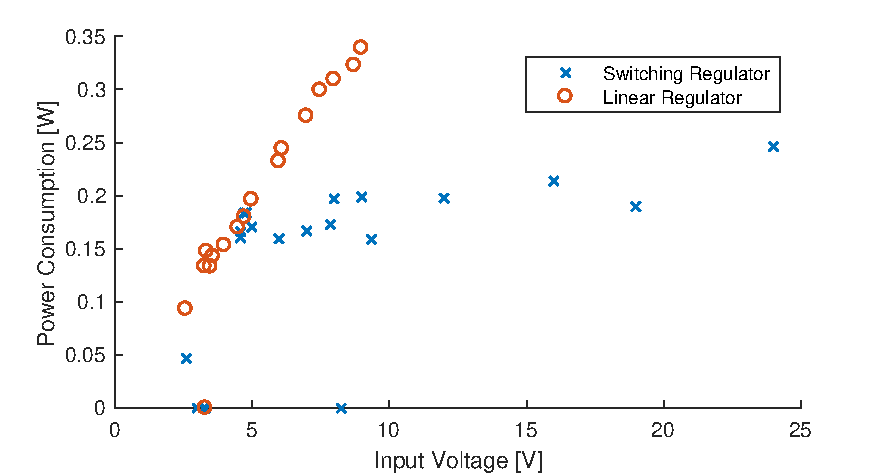
\includegraphics[width=1.0\textwidth]{src/switching_linear.pdf}
\caption{Comparison of the energy consumption between the linear regulator on the Arduino Pro Mini board and an external switching regulator}
\label{fig:switching_linear}
\end{figure*}

\section{Embedded Software}
The embedded software used on the transducer hardware was developed in the Arduino-specific C++ dialect. It was developed in using the visual micro (see \cite{vMicro}) plugin for Microsoft Visual Studio, but it can also be modified and built using the official Arduino IDE. 

The software is divided in two parts, the first one needs to be modified by users adapting the system to their needs while the second one is the technical basis that normally does not need to be modified. The code used for the demonstration device is included in the appendix of this document.

\subsection{Library Usage}
\subsubsection{GPS}
Most GPS-modules able to interface with Arduino software will do so transmitting so-called NMEA sentences (see \cite{NMEASentences}) via a serial interface. As this text-based format needs to be parsed into a format usable for retransmission of the relevant data portion there needs to be either a considerable amount of parser code included in the software or an external library used. As code readability, reusability and standard conformity can be significantly improved by using a library, it was decided a library should be used for the NMEA sentence parsing.

\paragraph{Adafruit GPS}
The Adafruit GPS Library (see \cite{AdaUltGPS}) is a library provided to be used with the Adafruit GPS module used in the demonstration assembly. There are however no official statements on compatibility with other GPS receivers and therefore this library is not considered to be a general solution for arbitrary GPS devices. 

\paragraph{TinyGPS}
TinyGPS (see \cite{TinyGPS} is a commonly used library for parsing NMEA sentences on the Arduino platform. It was written by Mikal Hart and is considered to be a good library for very restricted hardware environments.

\paragraph{TinyGPS++}
The TinyGPS++ (see \cite{TinyGpsPlus}) library is a spiritual successor of the TinyGPS library containing an enhanced set of features. The author recommends using it instead of TinyGPS in environments having enough resources to handle it. As program size is not a major concern for this embedded software, this library is used.

\subsubsection{Communications}
As a Bluetooth RFCOMM channel is used for communication towards the Android device, the microcontroller must interface with the Bluetooth module. This project uses transparent serial-pass-through Bluetooth modules and therefore there is no need for any interface library apart from the UART hardware interface code included in the Arduino core libraries.

\subsubsection{Data formatting}
The protocol specification (see \ref{sec:protocol}) stipulates the use of of the JavaScript Object Notation (JSON) as data transmission format for the serial communication towards the Android device. There is only one well-known Arduino library for JSON encoding which is called ArduinoJson (see \cite{ArduinoJson}) (the aJson library (see \cite{aJson}) cannot be considered an adequate alternative as it will not work on ATMega168-based boards). The library has a reasonably low memory footprint and allows for the creation of JSON Objects as proposed by the protocol specification.

\subsubsection{Sensors}
As the system specification allows for manifold sensor types and interfaces, normally some libraries should be used to collect the sensor data.

\paragraph{Demonstration Assembly}
\label{p:demonstration_device}
As the demonstration assembly contains two different sensor types, two libraries are used for sensor readout. The sensors are part of a proof of concept (as opposed to the main system components) and therefore the librarys used were chosen as first-that-fits. The libraries used are the \texttt{DHT Temperature \& Humidity Unified Sensor Library} (see \cite{DHTlib}) for the DHT11 temperature and humidity sensor and the OneWire (see \cite{OW}) and the DallasTemperature library (see \cite{DallasTemp}) for the DS18B20 One Wire temperature sensor.

\subsection{Basic Functionality}
In chapter (\ref{cha:requirements}) the basic requirements for the transducer device are outlined to be reading out sensors and sending it to the Android application.

\subsection{Sensor Readout}
The sensor readout needs to be adjusted to the type of sensor incorporated in the system actually build. Examples for sensor readout code can be found online for most common sensor models. The software especially focusses on sensors that allow one-shot readout, but code might be incorporated to support other readout mechanisms.

\subsubsection{One-Shot readout}
All code reading out the connected sensors and putting it in the JSON structure described in the protocol specification can be found in a single function that is called when the trigger button has been pushed or a measurement has been triggered through the Android application.

\subsection{GPS positioning}
The GPS receiver connection in the system might basically have three different states which must be handled accordingly.

\paragraph{No GPS Receiver or disabled}
If there is no GPS receiver included in the transducer hardware or the GPS receiver is disabled (which is a feature that might be implemented as a hardware switch or compiled into the software), there should be no position object included in the transmission data or the position object should only contain the isValid key. If the GPS feature is disabled during software compilation, the JSON message generated by the transducer should not contain a position object.

\paragraph{Waiting for GPS fix}
Normally a user should wait for the GPS position to be fixed before they trigger a measurement. If a measurement is triggered anyway, a position object containing only the isValid key should be sent to the Android device.

\paragraph{Position fixed}
When the position is fixed (and the age does not exceed a threshold of 15 seconds), a full position object containing the location information is included in the sentence.

\subsection{Additional Features}
\subsubsection{User Interface}
Apart from an LED that can be directly connected to the Bluetooth module to show its connection status, the software contains means to drive two status LEDs showing the GPS state and the state of a currently ongoing measurement. The GPS LED blinks while the device is on and there is no position fix and shows continuous light while a position not older than three seconds is available. The state LED for the current measurement is turned on when a measurement is triggered and turned off when an acknowledgement has been received.

\subsubsection{Resending Information}
\label{subsubs:resending}
\paragraph{Data Retention Mechanism}
The microcontrollers used in the Arduino Platform usually contain three different types of memory: SRAM, Flash and EEPROM. Normally the SRAM is used to store the data while it is processed and sent. However, the main downside of using SRAM is data loss in case of power loss or hardware resets. As both other memory types are non-volatile and thus retain their data also in case of a power loss, they are better suited for data retention purposes. The Arduino platform favors the use of the EEPROM memory by providing libraries and documentation. As also the lifecycle specified for the EEPROM is much longer, it is used for data retention in this project. The mechanism as implemented cannot be used on Arduino boards not equipped with an EEPROM like the Arduino Due. For these Boards, another mechanism based on a string buffer located in the SRAM has been developed. As SRAM is a volatile memory, the SRAM buffer cannot hold the data through power losses.

\subparagraph{Product Lifecycle Considerations}
As EEPROM allows only a limited number of write cycles, the overall product lifecycle must be considered when using EEPROM. A typical example lifespan of for the EEPROM included in an Arduino is the one from the ATmega328 (see \cite{ATmega328}) used in the demonstration device. It has a specified minimum lifecycle of 100 000 write cycles (after that often the data retention time will fade). A minimum lifecycle of 100 000 measurements is considered sufficient for the use cases proposed in this project.

\subsection{Performance Considerations}
When large libraries are used to handle the sensor data or there are many sensors connected, the SRAM space on the Arduino might be too small. In order to reduce problems that might arise from this, all constant strings in the code are encapsulated using the F()-Macro, which reads the strings from the program flash memory instead of transferring it into SRAM on startup.

\subsection{Fault Behavior}
Hardware and transmission faults might occur for unforeseen reasons and therefore the device should be able to handle these gracefully. This section covers the most common problems that might occur during operation.

\subsubsection{GPS Receiver}
As the GPS receiver might need a significant amount of time (about 30 seconds when there is no buffer battery) for the first position fix (or the fix is impossible due to obstacles blocking the signal), there is a significant period of time in which the device does not have valid location information. If a GPS status LED is incorporated, the user can wait until a position fix occurs or rely on the Android device to deliver location information. On the protocol side, a message is sent that contains a position object which only contains the isValid key and a false value. 

\subsubsection{Bluetooth}
Different Bluetooth modules might exhibit different behaviour regarding state pins exposed to the outside. Typically, the user can see a status LED showing the connection state in some way. If a measurement is triggered while there is no connection, the data is repeatedly resend (see \ref{subsubs:resending}) until an acknowledge is received from the Android device. If a new measurement is triggered before the data is acknowledged (shown by the state LED), the previous measurement might be lost.

\subsection{Extensibility}
Only standard Arduino hardware and software parts are used in this project, all extensibility options available for the Arduino platform might be incorporated into this system. This includes the use of software libraries, modules, shields and other electronic components.


\chapter{Android Application Software}
In order to receive, store, visualize and export the measured data generated by the system, an Android application has been developed.

\section{User Interface}
The application software was developed using an experience-driven model. The main objective regarding the user interface design was to build an app that does what the user expects. The functional logic has been designed to suit the user interface requirements. Experience-driven development lays a strong focus on the recognizability of user interface elements, which in turn means the app design mostly reuses design principles commonly used on the Android Platform. In order to reduce avoidable effort in design, it was decided to standardize the app on Material Design (see \cite{Material}). Material design is the native design guideline for Android versions newer than Lollipop (5.0) and also well-known on older devices, as many apps (including the Google apps) use material design also on older devices. The app tries to follow the Material Design Guidelines as close as possible in order to provide a familiar design to Android users. Most design elements are provided by the Application Support Library (see \cite{AppCompat}) which provides Material design components to old Android Versions back to Gingerbread (API 9).

\begin{figure}[ht]
	\centering
	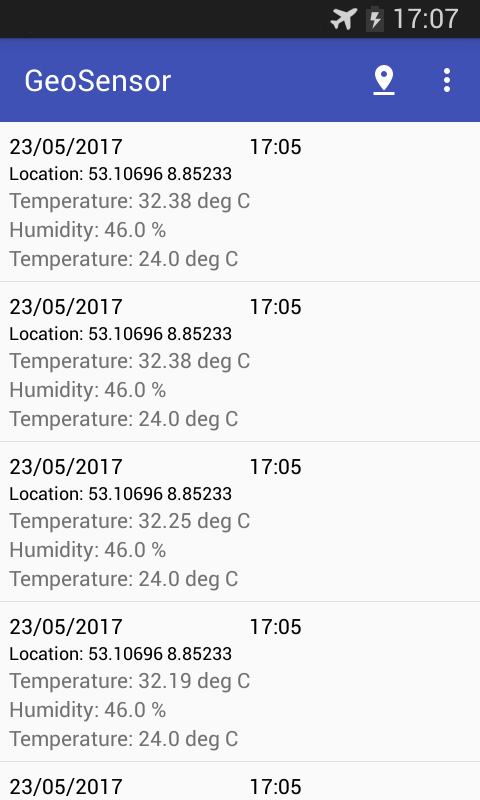
\includegraphics[width=6cm]{src/main_list}
	\caption[Main List]
	{The user interface of the main activity of the app as seen on a Samsung Android 4.2.2 device}
\end{figure}

\subsection{Internationalization}
As not every user feels comfortable using application software in foreign languages, the application is built to fully support localization leveraging the Android resource framework. The applications default language was chosen to be English (stylized as United States) as this is the fallback language international users normally expect in case there is no translation for their language. As a proof of concept and to be used by German-speaking users the app contains a full (meaning the user will not see any text in the default language) German (without further distinction by country) translation. As all user interface elements that might need a translation are included in the R.string resources, the app is prepared for further translations that might be added later. The app design includes the necessary preparations for right-to-left languages, but the compatibility for those languages is not a specific design target that. 

\begin{figure}
\centering
\begin{minipage}{.5\textwidth}
  \centering
  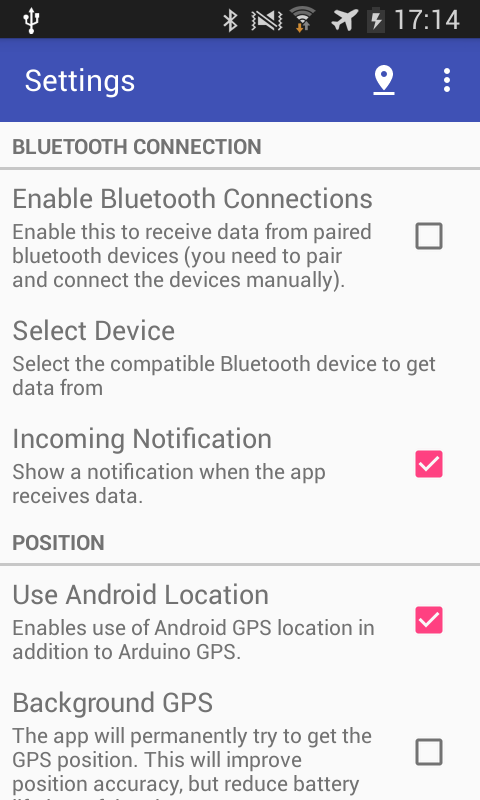
\includegraphics[width=.8\linewidth]{src/settings_en_1.png}
\end{minipage}%
\begin{minipage}{.5\textwidth}
  \centering
  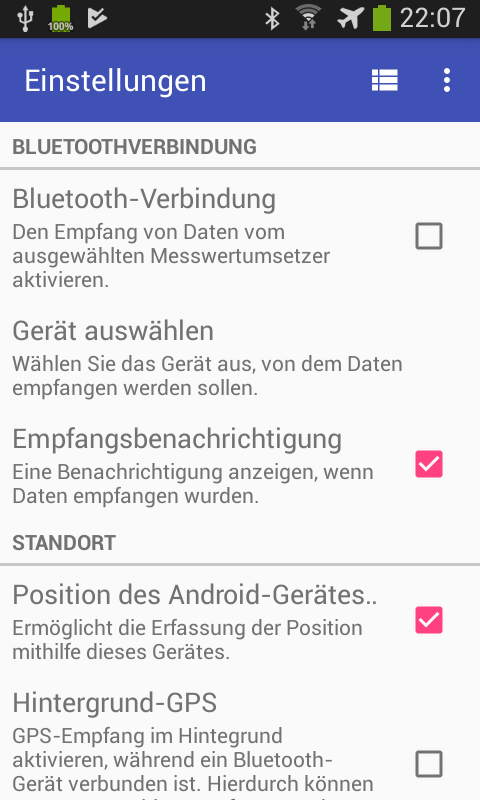
\includegraphics[width=.8\linewidth]{src/settings_de.png}
\end{minipage}
  \caption{Comparison of settings activity in the EN-US and DE-DE locales}
  \label{fig:settings_comp}
\end{figure}

In order to show the types of sensors in the user interface language, the app contains a mechanism to translate the measurement category to the user interface language. The mechanism uses a string array located in the resources to look up the localized denomination. If there is no translation defined, the measurement category is shown as it was transmitted by the transducer.

Times are always shown in the time zone the user has set the device to and formatted according to the local format given by the Android framework. An example of time formatting and sensor type translation can be seen in figure \ref{fig:lang_comp}.

\begin{figure}
\centering
\begin{minipage}{.3\textwidth}
  \centering
  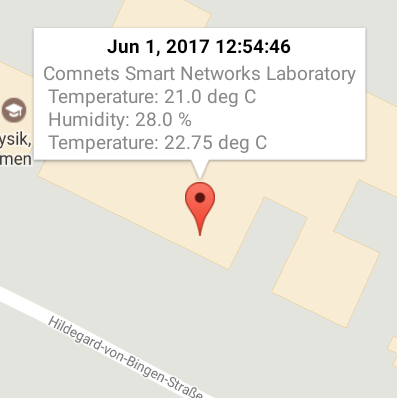
\includegraphics[width=.8\linewidth]{src/marker_en.png}
\end{minipage}%
\begin{minipage}{.3\textwidth}
  \centering
  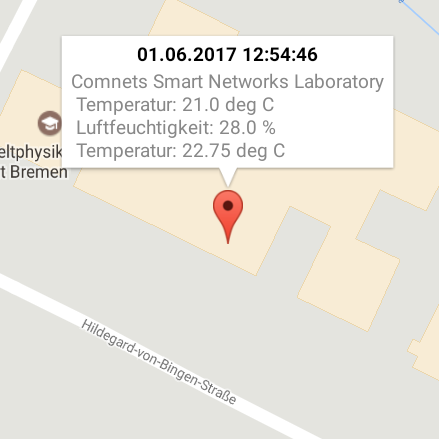
\includegraphics[width=.8\linewidth]{src/marker_de.png}
\end{minipage}
\begin{minipage}{.3\textwidth}
  \centering
  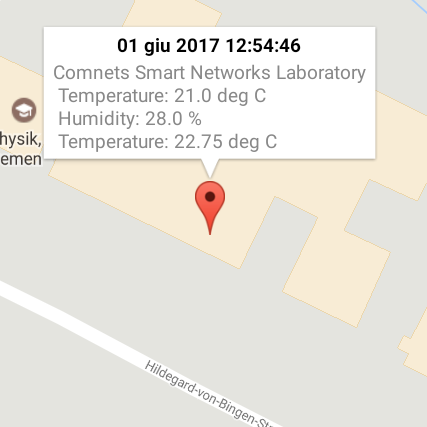
\includegraphics[width=.8\linewidth]{src/marker_it.png}
\end{minipage}
  \caption{Comparison of map marker contents in the en\textunderscore US, de\textunderscore DE and it\textunderscore SM locales.}
  \label{fig:lang_comp}
\end{figure}

\subsection{Toolbar}
Most Android apps use some kind of bar near the top of the screen to allow users to find the basic user interface elements. Often this bar is an \texttt{ActionBar} as provided by the Android framework. As this app is build using the Application Support Library the Toolbar provided by that library is used. The Toolbar contains the control elements needed in the specific Activity and changes accordingly. In most activities (if they are not designed to be modal) there is an overflow menu that contains any element overflowing from the Toolbar and the application settings. The material design guidelines specify that the application settings should always be shown in the overflow menu even if there would be enough space left for a button in the Toolbar itself.

\subsubsection{Export}
\label{subsubs:export}
In order to further process the data acquired by the system, the data can be exported. Even though the data model is object-oriented and contains lists of data which have variable length (the app does not have a priori knowledge of the sensors), the data export feature generates a comma separated values file (.csv-file) including the data acquired from the measurements. The table has a variable width as its width is adjusted to fit the number of sensors and the number of location objects associated with the measurements. The export can be configured to use decimal separators (period \/ full stop or comma) and field separators (comma, semicolon or tab stop) as needed. This setting is exposed in the application settings. Another option included in the application settings is to export only the best location associated with the data record which will make the structure of the exported file more regular as the first sensor will then always be found in the same column. The export however does not assert that the sensors will be exported in a specific order, which means in some cases the data will need to be ordered by an importing application (e.g. using the Excel LOOKUP function analyzing the imported data). The order of the exported sensors should however be consistent for the same transducer configuration. On large data sets the export might take some time, however the user can continue to use the app until the exported data is ready.

Old Android versions allow the App to directly write the export data to the so-called external storage on the Android device. When the export is finished, the app shows an alert containing the path (which is inside a folder called GeoSensor in the external storage root folder) of the exported file. The filenames of the exported file contain an export timestamp. Other apps or a USB connection can be used to open or move the file from the aforementioned folder.

\begin{figure}
\centering
\begin{minipage}{.5\textwidth}
  \centering
  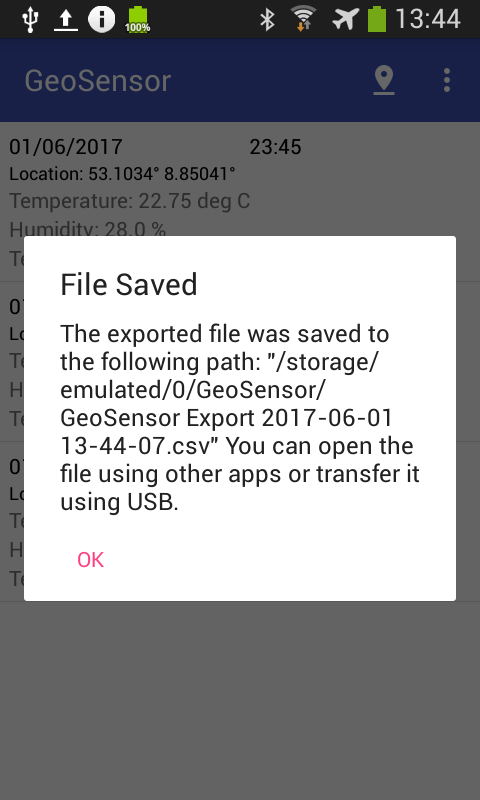
\includegraphics[width=.8\linewidth]{src/export_old.png}
\end{minipage}%
\begin{minipage}{.5\textwidth}
  \centering
  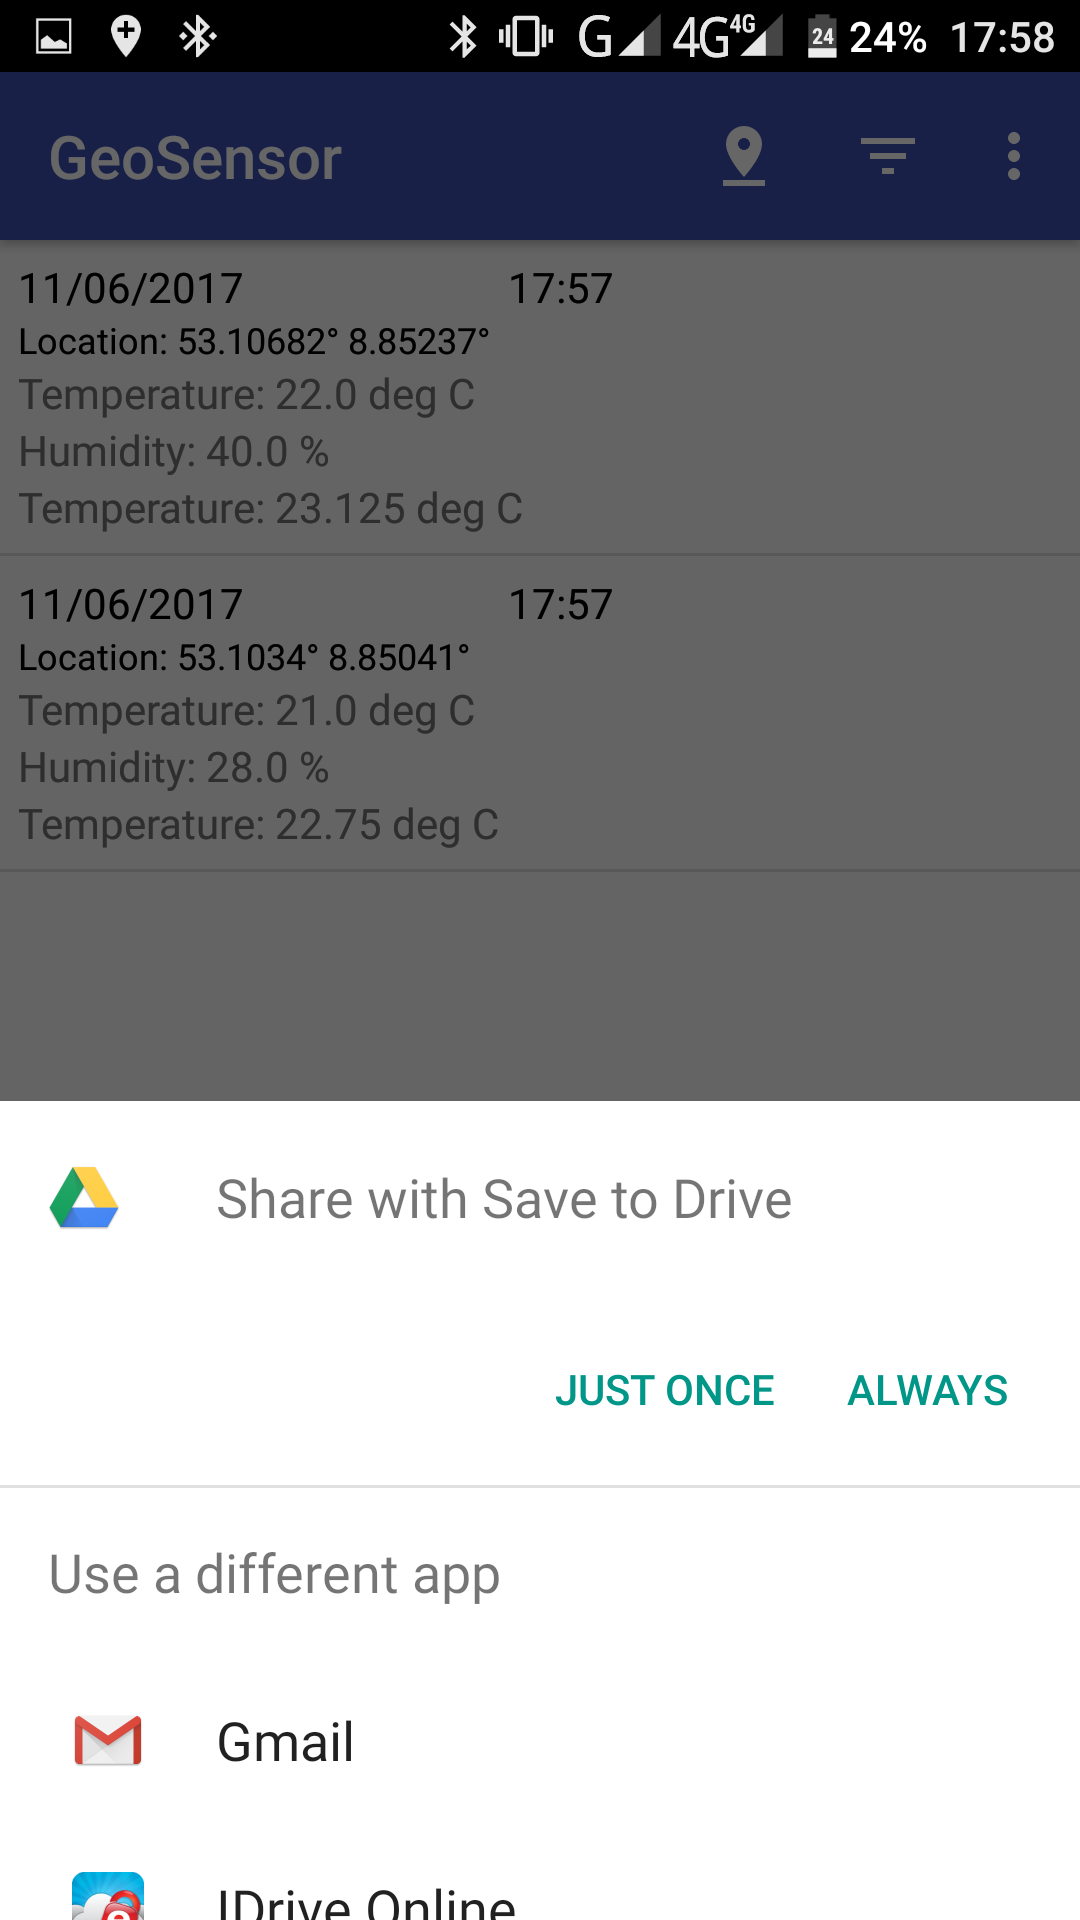
\includegraphics[width=.8\linewidth]{src/export_new.png}
\end{minipage}
\caption{Exporting data in older and newer Android versions}
\label{fig:export_old}
\end{figure}

\paragraph{Export after Android KitKat (4.4)}
In more recent Android versions the file handling works differently. After the data has been prepared, it is exported to an app that can handle general files which mostly includes cloud storage providers. The user is shown a system dialog asking him to choose the app to export the data to. In the dialog, there is a possibility to make the system open the app in the future again without asking. The app used for testing purposes is Google Drive as it is the most widespread cloud storage app in the Android ecosystem.

\subsubsection{Filtering}
\label{subs:filter-ui}
\paragraph{Filter by Time}
The time filter allows to choose a start and end time for the data records shown. The base time used for filtering is the receive time as that is guaranteed to be unique for each measurement data record and it exists for each data record. As the filter is set globally for the whole application, it applies to all views and also to exports. The setting however is not preserved across the application lifecycle which means it is reset when the application is closed. The filter logo changes to the accent color while a filter is deployed.

\subsection{First Start}
When the application is first started, the user is prompted to select a Bluetooth device the app should connect to. Note that as the app uses Googles auto backup feature where available, the application settings might be restored from a previous install if the app is reinstalled on the same device again or in case a backup was transferred to a new device. 

\subsection{Main List}
The main list is the entry point into the application. It is the main activity started first when the app is started. The main list contains a list element for each data record received from the database after applying the filter (see \ref{subs:filter-ui} and \ref{subsubs:filter-tech}). The element shows the receive time and date, the geographic coordinates and the measured values received. When the entry is touched, the details view (see \ref{subs:details-view}) is opened for the data record. When a new data record is received, the list refreshes automatically.

\begin{figure}
\centering
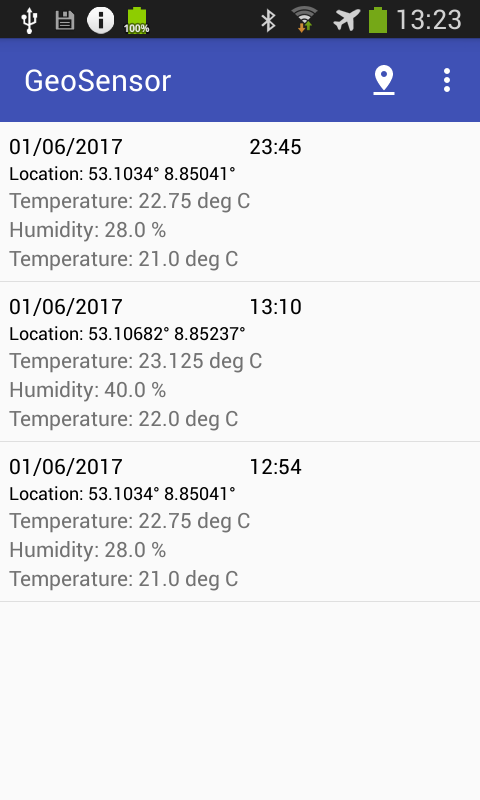
\includegraphics[width=.4\linewidth]{src/main_activity.png}
\caption{Main List View of the App}
\label{fig:main_activity}
\end{figure}

\subsubsection{Sorting}
The main list supports sorting the entries. On startup, the entries are sorted new to old by receive time. This default order was chosen as it allows to most recent and therefore probably most interesting data record to be seen on startup and also conforms to the order most social media services use for their information nowadays. There is a sorting button in the toolbar (or in the overflow menu if there is not enough space left in the toolbar) to select the sort order.

\subsection{Main Map}
\label{subs:mainmap}
Leveraging Googles Maps API (see \cite{GMapsAPI}), the app provides a map view in which every measurement is represented as a marker on the map. The map can be zoomed and rotated as a user familiar with the Google Maps app that is preinstalled on most Android devices, would expect. When a marker is tapped, an overlay window shows the measured values. The overlay can be tapped to show the details view for the respective data record. Filters work on the map the same as on the list. As the map is provided by the online Google Maps service, an internet connection is necessary to use the map view.

\begin{figure}
\centering
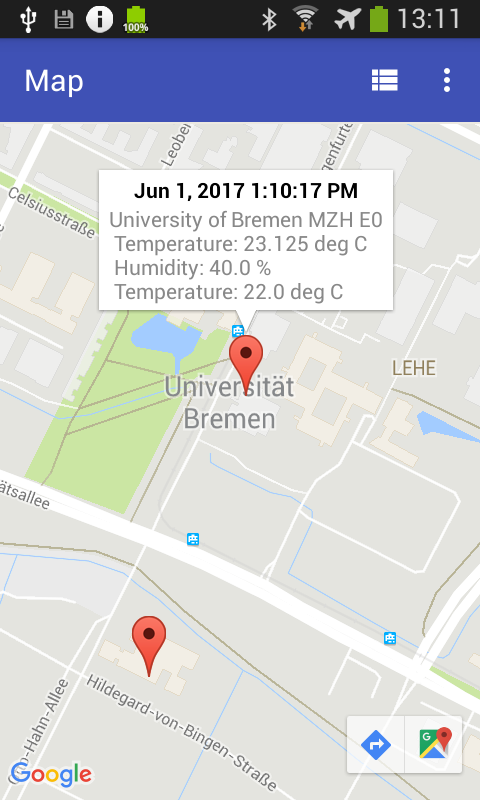
\includegraphics[width=.4\linewidth]{src/main_map.png}
\caption{Main Map View}
\label{fig:main_maps_view}
\end{figure}

\subsection{Details View}
\label{subs:details-view}
The details view is a card view (more information about the card view design pattern can be found in the Material Design Guideline \cite{Material}) showing all information available regarding a data record. It contains a card for every location associated with the data record (which might be more than one in case the transducer has a GPS receiver and the Android device location is switched on as well), a card showing all the associated locations on a map and a card for each measured sensor value.

\begin{figure}[h]
\centering
\begin{minipage}{.33\textwidth}
  \centering
  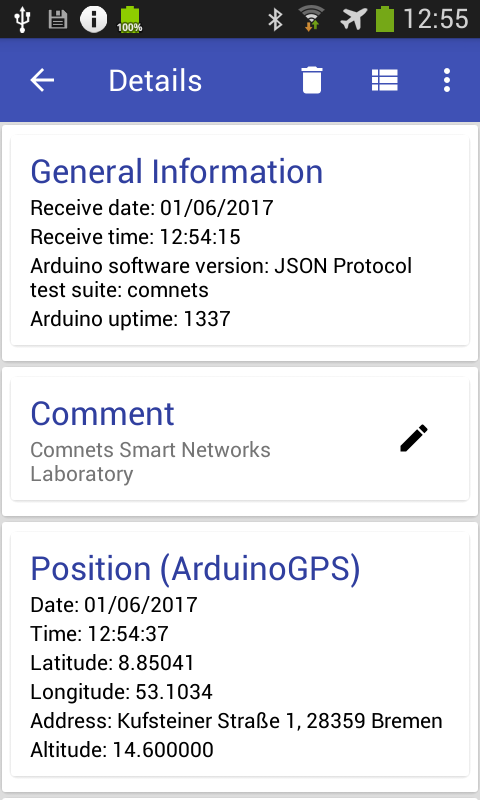
\includegraphics[width=.95\linewidth]{src/details_1.png}
\end{minipage}%
\begin{minipage}{.33\textwidth}
  \centering
  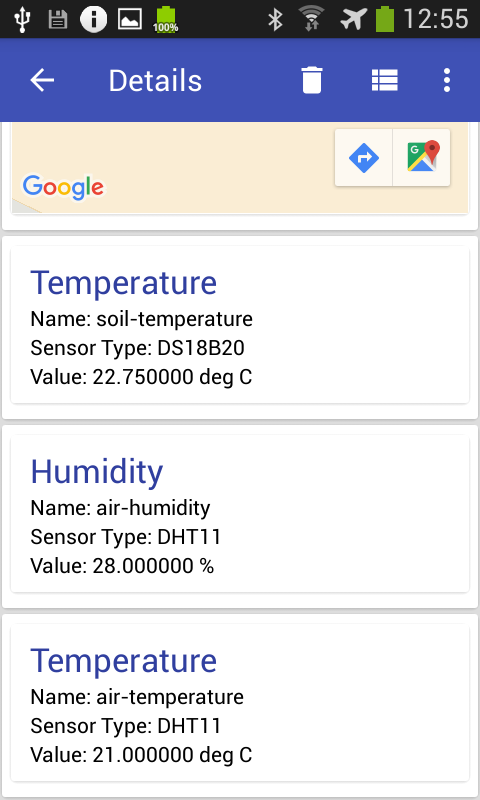
\includegraphics[width=.95\linewidth]{src/details_2.png}
\end{minipage}
\begin{minipage}{.33\textwidth}
  \centering
  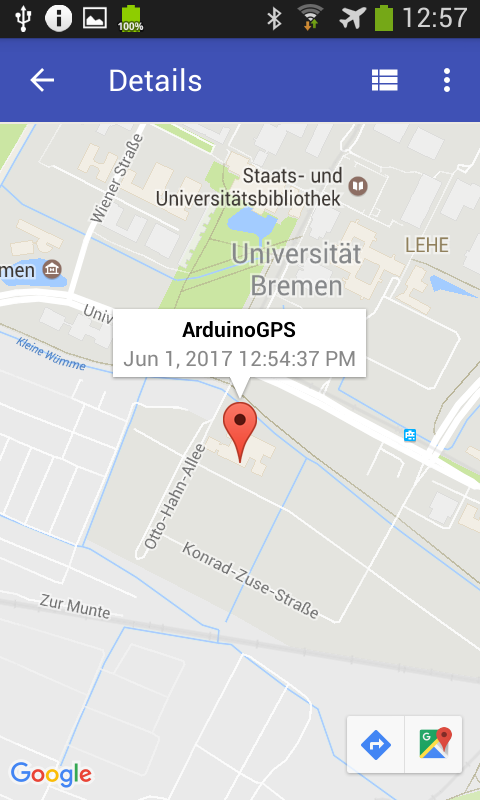
\includegraphics[width=.95\linewidth]{src/details_map.png}
\end{minipage}
  \caption{Details View}
  \label{fig:details_view}
\end{figure}

\subsubsection{General Information}
The general information card contains all the information included in a message of the protocol but not related to a sensor or the location. This includes the embedded software version deployed on the Arduino, the time when the data record was received and the uptime of the Arduino device when the message data was build.

\subsubsection{Comment}
The comment is a string that might be changed by the user. It is initially sent by the transducer device and can be modified in the app. In order to modify the comment, the user needs to touch the pencil icon on the comment card and he will be able to modify it in an alert dialog. The comment is included in the export data and therefore must not contain the field separator used in the export files. As a rule of thumb all three possible separator characters should not be included in the comment. As the export files do not specifically use an extended character set it is also advisable to use only characters contained in the ASCII-charset in the comment field.

\subsubsection{Location Data}
For each location that is associated with the data record, a separate card is shown. While all other views only show the best location available for the data record, all locations are shown in the details view. The card contains all available location information like altitude and precision if they have been included by the location provider. Data fields that are not available are not shown. If an internet connection is usable, Googles reverse geocoding API is used to provide a human readable street address for each location.

\subsubsection{Map}
As the main map view (\ref{subs:mainmap}), the details view uses Google Maps to show a map containing a marker for each location associated with the data record. For performance reasons the card only shows a static map. If the user wants to see an interactive map, they can tap the map and get an activity containg a full map. If there is no internet connection available to load the map, this card is not shown.

\subsubsection{Measured Values}
Every measured value transmitted according to the protocol (as defined in \ref{sec:protocol}) consists of five data fields which are shown in this card. All measured values have separate cards even if they have the same measurement category or are derived from the same sensor.

\subsection{Settings}
The application settings can be reached using the overflow menu in one of the activities. They are grouped into different categories (preference groups).

\subsubsection{Bluetooth Connection}
The Bluetooth connection category contains some of the most important settings for the app. 

The first setting switches the Bluetooth connection to the transducer device on or off. If this setting is on, the app will continuously hold a connection to the transducer device or be searching for a transducer device. As this requires Bluetooth, in newer Android versions the according runtime permission is requested when the Bluetooth connection is switched on. If Bluetooth is switched off in the system settings or the quick settings, the user is prompted to activate Bluetooth.

The second setting allows the user to select the Bluetooth device to which the app connects. When tapped, a list of all the paired Bluetooth devices is shown. The user should pair the Bluetooth device beforehand as programmatically coupling a device might lead to unforeseen problems (it however in general is possible). Coupling a Bluetooth device in Android is an undocumented function that can however be used acquiring a function handle using the Reflection API. The User then sees a dialog asking them to input the key needed for pairing. Under the list, a button is shown which allows the user to search for Bluetooth devices not paired yet. The devices are added to the list shown as they are found. If the user chooses a device from that list he should be shown a dialog asking him to pair the device.

The third option allows the users to choose if they want to be notified when a new data record is received. If the option is active a big text notification including the measured values is shown every time a data record is received. In order to not spam the notification area, any old notification is automatically replaced by a new one and thus at most one notification is shown.

\subsubsection{Position}
As defined in \ref{sec:location}, the app can record a position for the data records even if the transducer device does not contain a GPS module. The user has two options that can be activated in this section. The first one allows them to use a low energy method provided by Google to fix the location after a data record has been received. In slow moving applications, this approach should be sufficiently fast. The second option allows them to activate background GPS while the app is connected to the transducer. While background GPS is enabled, high accuracy positions are available as long as there is sufficient GPS signal reception. The GPS only feature might work on devices that do not provide Google libraries even though those devices are not part of the target device group for this app. The accuracy and speed if the first method is greatly improved while background GPS is activated.

\subsubsection{Data Export}
In the data export category the user can chose the decimal mark and the column separator for the export files. This is necessary as different programs have different requirements for data imports. A German version of Microsoft Excel for example needs a comma as decimal mark and a semicolon as column separator while Matlab needs a period as decimal mark and a comma as column separator. As described in (\ref{subsubs:export}) the third option allows to only export the best location available for each data record.

\subsubsection{Data}
The database section contains two options to allow basic database handling. One option lets the user chose a threshold date and cleans all older data records, the other one drops all contents of the database.

\subsubsection{Transducer Device}
In the transducer device section a message resend from the transducer device can be triggered.

\subsection{Miscellaneous Features}
\subsubsection{Automatic Database Backup}
On devices running Android 6.0 Marshmallow or newer, the app leverages the auto backup capability offered by the Android System and Google Drive. Auto Backup is a service meant to provide zero-configuration application backups. If the user uses Google Drive, the application database is regularly backed up to Google Drive. When the application is reinstalled (which would normally delete the application data on the device) the auto backup mechanism might restore the old database.

\subsubsection{Application Logo}
The application logo is a map marker in a yellow circle. It is shown in figure \ref{fig:logo}.

\begin{figure}[h]
\centering
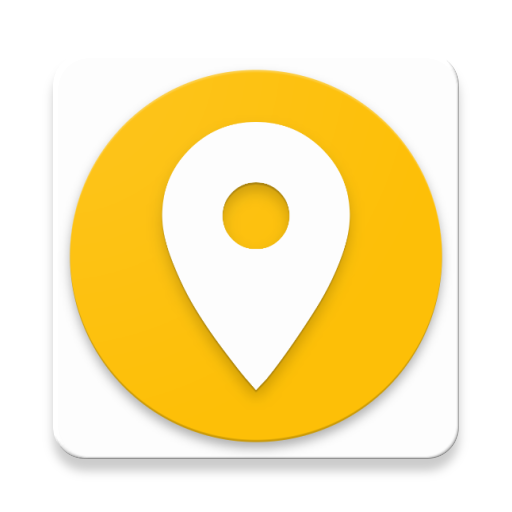
\includegraphics[width=.2\linewidth]{src/logo.png}
\caption{Application Logo}
\label{fig:logo}
\end{figure}

\subsubsection{Bluetooth Status Notification}
When the app is either searching for the selected Bluetooth device or connected to it, a notification is shown in the Android status bar. This notification enables the user to be actively aware of the state of the app even when the app is not running in the foreground. At the same time, a foreground notification gives the service a higher priority which means it is less likely to be stopped by the Android system. A tap on the notification leads to the application settings while the app is searching for the chosen device as this facilitates turning off the connection or changing the device to connect to. While the app is connected, tapping on the notification leads to the main activity and therefore to the most recent measurements received.

\begin{figure}
\centering
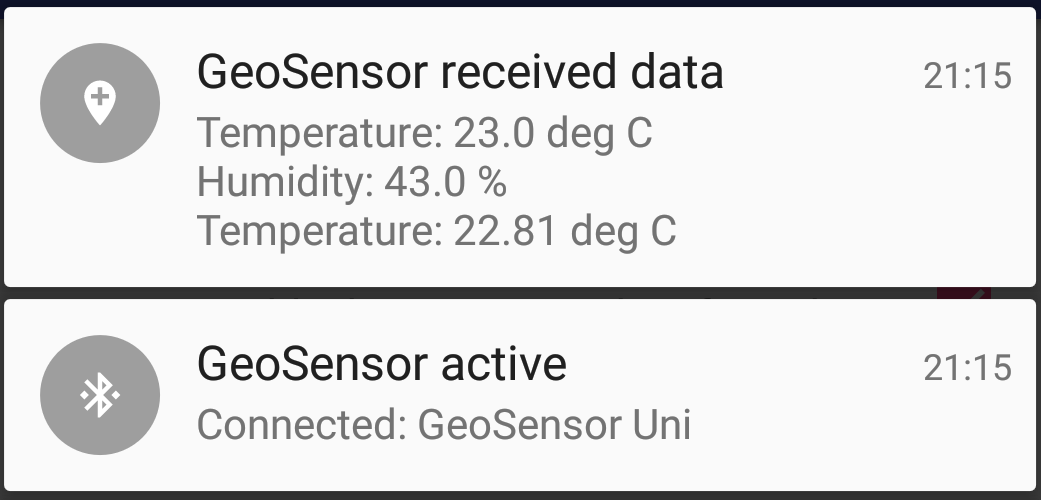
\includegraphics[width=.4\linewidth]{src/notification.png}
\caption{Notification as seen on Android 6.0 Marshmallow}
\label{fig:notification}
\end{figure}

\section{Backend}
Like most Android Apps, the app is written in the Java Programming Language (see \cite{JavaSpec}). The code was developed in Android Studio (see \cite{AndroidStudio}) and can be build using the Gradle build system included in Android studio.

\subsection{Dependencies}
Apart from the Android Platform itself (the app is built for target SDK version 25), the app does use two other libraries to provide core functionalities.

\subsubsection{Android Support Library}
The app uses the following modules of the Android Support Library (see \cite{AppCompat}) in order to provide the material design components used for all supported versions of Android:
\begin{itemize}
\item com.android.support:appcompat-v7
\item com.android.support:preference-v7
\item com.android.support:cardview-v7
\item com.android.support:design
\end{itemize}

\subsubsection{Google APIs for Android}
In addition to the Android APIs, the app uses two libraries provided by Google, which are available on Android devices equipped with the Google Play Store. 

\paragraph{Fused Location Provider API}
The Google Location Services include the Fused Location Provider API. This API offers an additional abstraction layer for the Android Location API. It combines information derived from different hardware resources into a single API that delivers the best results available at the time of the request. For example, this API might provide a WiFi-Based position when indoors and aggregate information derived from the GPS, GLONASS, Baidu and Galileo satellite navigation systems depending on which of these are available on the respective device. 

\paragraph{Google Maps API for Android}
As the app should visualize the location of the measurements on a map, the app needs a map. As including an offline map into the app would take an unreasonable or even unfeasible amount of storage space, the app needs to use online maps. On the Android platform, the most common provider for maps is Google and therefore users typically expect to see a Google Map where a map is needed. Apart from the map itself, the API includes a reverse geocoding function that can be used to retrieve a nearby human-readable street address for a given geographical location.

\subsection{Class Structure}
\subsubsection{Activities}
As most Android applications, this app is made of multiple activities. All activities in the app are derived from the GeoSensorActivity which in turn is a chile of AppCompatActivity. This allows the activities to contain a Toolbar (also from the Support Library) as action bar and follow the material style on all supported Android versions. While the toolbar used is the same in all activities, the activities show different action items in it and the selection of option items in the Toolbar is handled exclusively by the Activity showing it.

\subsubsection{Helper Classes}
The application contains helper classes for different tasks. The function of the helper classes is explained in the following subsections ordered by their role in the app.

\subsection{Bluetooth Communications}
\label{subs:bt-tech}
The Bluetooth communications are handled by a service class named BluetoothReceiverService. The service has 5 distinct states and a well-defined set of transitions that might occur between these states. The following paragraphs explain the states and the possible transitions between them. The state variable set to initialising when it is created (i.e. before the constructor and the onCreate lifecycle method are called). The service continues to run in any state until it is stopped by the framework (typically due to low memory or because the user actively closed (not just suspended) the app.

\paragraph{Initializing}
The initializing state is the first one when the service is started. During the initialising state the constructor and the onCreate lifecycle method are called by the Android framework. These methods mostly register broadcast receivers for the Bluetooth status broadcasts, some application internal broadcasts and a listener for application setting changes. After that, the service tests, if the application settings have been correctly set. If not (which should be the case only on first start), the FirstStartActivity is started in order for the user to choose the Bluetooth device to connect to. Then the service determines if the Bluetooth connection is enabled in the application settings. If it is not, it will go into the disabled state after the initialization process for the Service is finished. If the connection is enabled in the application settings, but Bluetooth is disabled, an intent asking the user to enable it is started and the state is set to \emph{Bluetooth off}. Finally if the initialization is finished, the connection is enabled and Bluetooth is available, the state is changed to \emph{searching}.

\paragraph{Bluetooth off}
The service does not do anything besides listening for broadcasts while Bluetooth is switched off. If Bluetooth is enabled by the user (often as a result of an intent asking them to do so), the service determines if the connection is enabled in the application settings and changes to the \emph{disabled} state if it is not and to the searching state if it is. 

\paragraph{Disabled}
This state is used when the Bluetooth connection is disabled in the application settings. The service continues to listen for preference changes and switches to the searching state when the correspondent setting is enabled.

\paragraph{Searching}
In the searching state the service will regularly try to connect to the transducer device chosen by the user. As waiting for a Bluetooth connection is a long-running task, the connection attempts are carried out in a different thread. As the task should not be interrupted by the system, it shows an ongoing notification and informs the Android system it runs in the foreground (i.e. it is a service the user is actively aware of). While the Bluetooth connection is searching, it retries to establish a connection about five seconds after a failed connection attempt. If the connection is established, the state is changed to connected. The other state transitions that might occur are to Bluetooth off if a broadcast is received and to disabled if the user changes the preferences.

\paragraph{Connected}
While the transducer device is connected, the service employs a thread which is constantly polling the communication channel for new bytes received. The incoming bytes are put into a string buffer and given to the parser function if the end of text (0x03) character is detected. In the connected state messages can be send to the transducer device. A state transition from the connected can occur to the Bluetooth off and disabled states for the same reason it would occur from the searching state and to the searching state if the connection is lost. A connection loss is detected through the system-wide ACL disconnected broadcast. This broadcast announces a connection loss in the link layer protocol. The ACL (asynchronous connection-less) link layer protocol typically waits 20 seconds after the last message until it considers a connection lost, under normal conditions the radio frequency communication (RFCOMM) protocol used uon top of ACL keeps the connection alive.

\subsubsection{Service Interface}
The Bluetooth stack was designed to specifically suit the requirements of the transducer device designed for this thesis, therefore only little interaction is needed. The user can use a button to trigger measurements and use the application settings to change the transducer device to connect to and deactivate the Bluetooth connection. The communications between other app components and the service uses a listener for changes in the applications shared preferences and broadcast receiver for all other communications within the app. Broadcasted intents are used for communication both towards and from the service. Other components might broadcast an intent containing the string \texttt{acquireMeasureData} if they want the service to transmit a signal requesting a measurement from the transducer and containing \texttt{resendMeasureData} if they want to trigger a resend. 

An intent is broadcasted from the service to notify other parts of the app when a new data record has been received. This intent contains the string \texttt{dataRecordReceived}.

\subsection{Data Backend}
The data backend uses a SQLite database to store the data at rest and an object-oriented approach to handle the data while the app is used. The SQLite version included in the respective Android platform is used to handle the data saved to the database which is named \emph{MeasureData.db} and saved in the applications private data directory. As the database resides in the private storage directory of the app, it is automatically backed up by the \emph{Auto Backup for Apps} technology (see \cite{Backup}) on recent Android versions. The database model closely resembles the data object model used in the app and can be found in figure \ref{fig:database}.

\begin{figure*}[h]
\centering
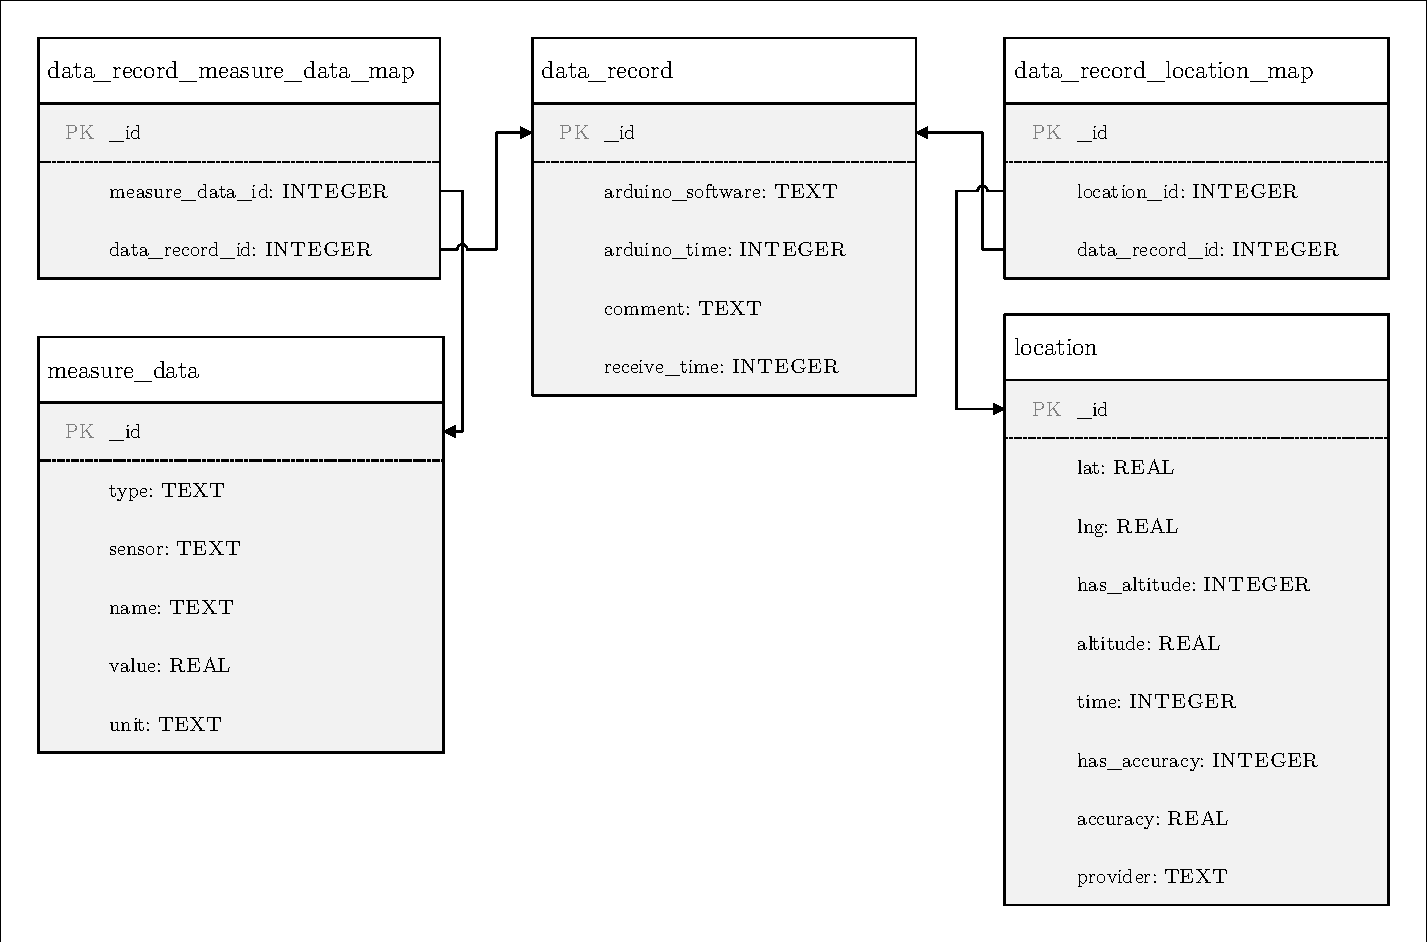
\includegraphics[width=1.0\textwidth]{src/database.pdf}
\caption{Database Model}
\label{fig:database}
\end{figure*}

All database handling in the app is done by instances of the DataLab class. The DataLab class provides all means necessary for the conversion between database data at rest and the objects used in the other parts of the app. Additionally it also includes the methods used to parse the incoming data from the JSON messages received.

\subsubsection{Data Objects}
The object-oriented data model used while the data is shown is based on the DataRecord class. For every measurement that is handled in the app a data record object is used. All data fields in a data record except the comment are immutable not only during the object lifecycle, but from the time they are first inserted into the database. The same data can be read into a DataRecord object multiple times and therefore identical copies might exist. If the comment is changed, it is immediately written into the database but other copies that exist at the same time are not affected. As a data record might include the measurements of different sensors, the sensor data for each value read from a sensor is saved in a separate object of the MeasureData class. The data record object contains a list of MeasureData objects associated with it. MeasureData objects are immutable. The data record also contains a list of Location objects including the location data derived from different sources. For reference, the information contained in the different data objects is:

\begin{itemize}
\item DataRecord
\subitem List of the associated measure data objects
\subitem List of the associated geographic locations
\subitem The time it was received (based on the Andoroid clock)
\subitem The uptime of the Arduino system when the data was sent.
\subitem The (user-editable) comment
\subitem The unique ID used in the database
\item MeasureData
\subitem The measurement category
\subitem The sensor type used
\subitem A name given for the sensor
\subitem The numerical measured value
\subitem The unit of the measurement. 
\item Location (the Location class is part of the Android framework, but only the properties mentioned here are put into the database)
\subitem Latitude
\subitem Longitude
\subitem Altitude
\subitem Time
\subitem Accuracy
\subitem The location provider used
\end{itemize}

\subsubsection{Data Parsing}
Data transmitted from the transducer device to the app is according to the protocol specification encoded in the JavaScript Object Notation (JSON) and can therefore easily be converted into Java objects. The contents of the JSON message directly correspond to the object structure used in the app. The structural JSON parsing itself is done by the \texttt{org.json} library included in the Android platform. The parsing code can be found in the DataLab class.

\subsubsection{Database Model}
As all data objects (except for the lists of other objects) contain a constant set of data fields, they can easily be represented as rows in a relational database layout. This means there is a table for DataRecord objects, one for MeasureData objects and one for Location objects. There are separate tables mapping the MeasureData and Location entries to the DataRecord objects. While adding the primary key of the DataRecord object to the Location and MeasureData tables as foreign keys, this solution is more versatile regarding future changes as it allows many-to-many relations.

\subsubsection{Filtering}
\label{subsubs:filter-tech}
Filtering by time is a feature directly derived from the database engine. As the database stores the time as an integer timestamp, both a lower and an upper limit can easily be included into the SQL-query.

\subsubsection{Sorting}
Much like filtering by time, sorting by time is a feature directly taken from the database engine.

\subsubsection{Deleting Data}
Besides the possibility to delete a single data record available in the details view, the application settings expose the option to delete old items or to drop the whole database. If the user chooses to drop the database, all tables are dropped and created from scratch again, if only old data should be deleted, the database is queried for all data records including a timestamp older than the user-chosen threshold and deletes these using the delete method for single data records which also follows the mappings in order to delete the associated location and measure data entries.

\subsection{CSV Export}
\label{subs:csv_export}
The comma separated values (CSV) export feature has been specifically designed for this app and does not use any libraries apart from the standard Java string handling. If a CSV-file should be saved, the CSVWriter generates a column layout that has enough space for all locations and measured values included in any of the data records exported. The data records to be exported are given to the CSVWriter class as a list of the DataRecord's database IDs. The CSVWriter loads all DataRecords into memory and generates a string containing all information included in the data record and formatted according to the columns generated for this export. As the export should be as versatile as possible, the user can choose their preferred decimal mark (either a dot / full stop or a comma) and value separator (comma, semicolon or tab stop). The table is then concatenated line-by-line and saved to the filesystem. On Android versions before Android 4.4 KitKat (API level 19) the file is saved to the public storage of the phone and can be opened by other apps or transferred to a computer using the USB connection. When the exported file is ready, an alert dialog is shown. On devices running Android KitKat or newer, a file provider is used to grant access to the data to a third party application handling files. When the file is ready, the user is asked to choose an app to handle the data. Typically cloud storage providers offer to take such data and save it to their clouds. For development purposes Google Drive is used as the reference cloud storage provider, but others like Microsoft OneDrive and Dropbox should work as well. A major advantage of this method is that there are no copies of the data permanently residing on the Android device as the app can delete it's copy of the data immediately after the export is completed.

\subsection{Positioning Strategies}
\label{subs:geolocalisation_strategies}
Apart from the position data provided by the transducer device, the application software enables the system to record location data provided by the Android system software. There are two different methods used for positioning which do however interact.

\subsubsection{Android GPS Location Provider}
Most Android devices contain an embedded hardware GPS receiver. If they do, a location listener can be employed to get location updates from this sensor. Typically, GPS sensors do provide a high location accuracy (between four and 20 meters for a 68 \% \/ $1~\sigma$ confidence interval) but do need good signal reception and a long startup time. As waiting a long time (often between 30 seconds and two minutes) before the location is recorded is unacceptable in most use cases, the GPS receiver must be activated before the measurements are triggered. While the Android GPS Location Provider is switched on in the application settings, the Bluetooth receiver service registers a location listener that gets regular location updates while there is a Bluetooth connection to the transducer device.

\subsubsection{Google Fused Location Provider} 
The Fused Location Provider provided by the Google Play Services on Android devices equipped with the Google Apps (which are virtually all commercially available devices outside of China) offers information derived from different sensors. While the API is similar to the one employed by the GPS location provider the fused location provider typically delivers high accuracy results much faster than the GPS location provider. In order to avoid unnecessary power consumption, the fused location provider is therefore is activated to get the location only when a data record has been received. There is a class called \texttt{DelayedLocationProvider} that is used to get the first high accuracy position when it is ready. If after 40 seconds no high accuracy location can be fixed the fused location provider is asked to provide the best location possible even if is low accuracy or outdated. 

\section{Software Quality}
While users of other platforms are often forced to use software that does not work as expected and needs workarounds to be known by the user, users of mobile platforms typically expect application software to \emph{just work}. Furthermore, the Android platform proposes a set of core app quality criteria (see \cite{CoreAppQ}) an app can be tested against. While most criteria should be met \emph{by design}, this section documents considerations about the criteria that are not completely met.

\subsection{Libraries}
The app includes and slightly outdated version of some libraries in order to support the Android API level 9. If the newest versions would be used, as of May 2017 the minimum API level would need to be elevated to 14.

\subsection{App State}
Being ready to receive data via Bluetooth even while the app is in the background is considered a core capability of the app and therefore does not violate the FN-S1 quality rule defined in the core app quality guidelines.

\subsection{Known Issues}
\subsubsection{Vector Drawables}
There is a problem using vector drawables as notification icons on versions of Android prior to 5.0 Lollipop. In these versions, other icons taken from the Android class are used.

\subsubsection{Zooming in Google Lite Maps}
The map used in the details view might in some cases exhibit strange zoom levels. This behaviour has been reviewed but no solution has been found. When the map is clicked, the larger map shown does however show normal behaviour.

\chapter{Testing}

\section{Transducer Device}
As all the functions provided by the transducer device are part of the overall system, the transducer device actually build as demonstration device is tested implicitly in the system tests. This section only covers additional tests that do not directly regard the usability of the demonstration device.

\subsection{Embedded Software}
Most parts of the embedded system software will be tested implicitly in the system testing part, but there are some specific features included in the software that need to be tested separately as they are not used in the demonstration device.

\paragraph{Using an SRAM buffer for resending}
This feature was tested on an Arduino Due microcontroller board as this board is equipped with a higher amount of SRAM allowing the message to be stored in SRAM. At the same time it is a board that does not contain EEPROM and therefore needs to use SRAM or Flash if a resend feature should be available. The only code modifications necessary in comparison to the demonstration device are commenting out the EEPROM\textunderscore RESEND define and defining SRAM\textunderscore RESEND. This system was only tested in order to show the software capability to resend data saved in SRAM. The function has been found to work without any problems.

\paragraph{Using a Hardware Serial for the GPS module}
For this test an Arduino Due has been used as this board contains four hardware serial ports. The software modification needed for this change is commenting out the GPS\textunderscore SOFTWARE\textunderscore SERIAL define and defining GPS\textunderscore SERIAL as the serial port used. There were no problems discovered during this test.

\paragraph{Fault Behavior (resending)}
As the system normally does not produce fault conditions triggering the transducer device to leverage its resending capabilities, this feature is tested separately. There were some test cases created used to test the resending behavior of the transducer demonstration device (which is using the EEPROM as a resending buffer):
\begin{itemize}
\item The pin used transfer information from the Bluetooth module to the Arduino was disconnected. A resend every 5 seconds is expected.
\item The trigger is pushed while the Bluetooth function is disabled in the app. When Bluetooth is reactivated, receiving the message on the Android device should take at most 5 seconds.
\item The resend option in the application software settings is used. The occurence of two data records distinct only by the receive time is expected.
\item The trigger is pushed while Bluetooth is switched off on the Android device. After the measurement, the transducer is turned off. While the transducer is turned off, Bluetooth and the app are activated on the Android device. The expected result is receiving the data as soon as the transducer is turned on.
\end{itemize}

All these tests were carried out and the expected behavior was fulfilled in all cases.

\subsection{Energy Consumption}
As a multitude of different sensors and microcontrollers might be used in the transducer platform, no conclusive statement regarding the energy consumption can be made. However the energy consumption can be probed using the demonstration device described in section \ref{p:demonstration_device}. The demonstration device allows two modes of operation including and excluding the GPS receiver and it's active antenna. The energy consumption has been measured feeding the system through the linear voltage regulator and feeding it directly inputting 3.3 V into the regulated voltage part. Even though current spikes might be observed while searching for Bluetooth devices, reading sensor values and reading or writing EEPROM, the major factor in the system is considered to be standby current draw. Recording the current and voltage output of a HAMEG Instruments HM8143 power supply some values power consumption data was acquired for the whole system and some of its most exposed parts. During all the measurements, each input channel was smoothed by a 1000 $\mu F$ capacitor inserted in the input channels next to the main consumers (the GPS module and the Arduino board).

The standby current can be considered mostly stable and the averages recorded after the startup phase were:
\begin{center}
  \begin{tabular}{ | c | c |}
    \hline
    Arduino Microcontroller, Sensors and Bluetooth module (connected) & 7.7 mA \\ \hline
    GPS module without external antenna & 22.0 mA \\ \hline
    GPS module including external antenna &  31.9 mA \\
    \hline
  \end{tabular}
\end{center}

The data recorded for the GPS module and the antenna approximately coincide to the values stated in the documentation (20 mA for the module, see \cite{AdaUltGPS} and 10 mA for the antenna, see \cite{ExtAnt}).

On startup and while measure data is acquired and sent, the power consumption is somewhat higher, the current draw of the basic system with the GPS connected to a different channel during the operations is shown in figure \ref{fig:startup_current} and figure \ref{fig:send_current} 

\begin{figure*}[ht]
\centering
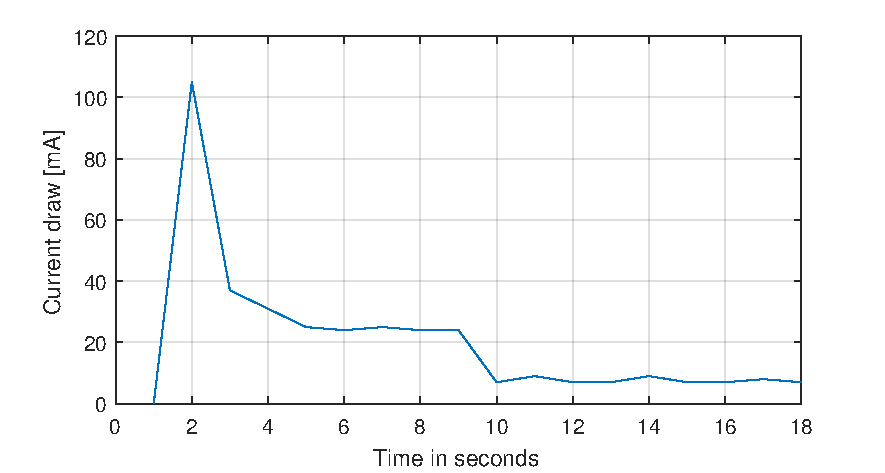
\includegraphics[width=1.0\textwidth]{src/start_current.pdf}
\caption{Current draw on system startup (without GPS)}
\label{fig:startup_current}
\end{figure*}

\begin{figure*}[ht]
\centering
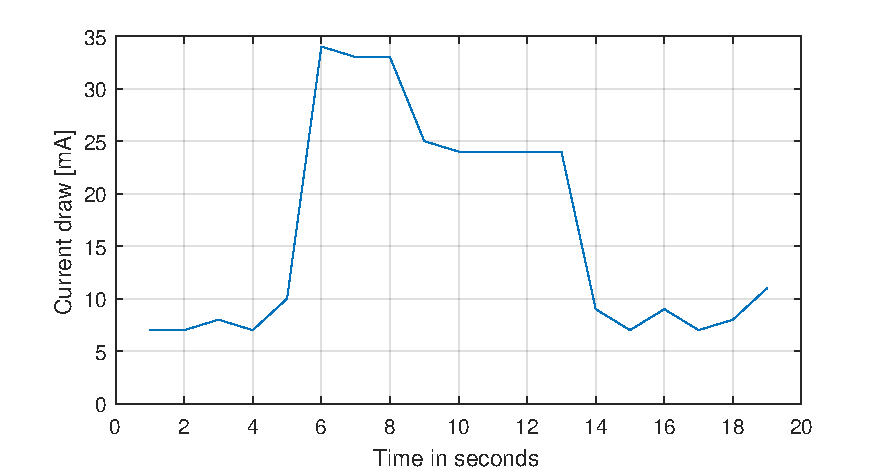
\includegraphics[width=1.0\textwidth]{src/send_current.pdf}
\caption{Current draw after a measurement has been triggered (without GPS)}
\label{fig:send_current}
\end{figure*}

\section{Application Software Testing}
\subsection{Core App Quality}
The application software was tested against the Core Suite test procedure of the Android Core App Quality guidelines (see \cite{CoreAppQ}). The test devices used in this test were the following:
\begin{itemize}
	\item An Ulefone Power running Android 6.0 and patch level September 5th 2016
	\item A Samsung Galaxy S III mini running Android 4.2.2 Jelly Bean
	\item A Sony Xperia Go running Android 2.3.3 Gingerbread
\end{itemize}

The following issues have been uncovered and resolved in the testing phase:
\begin{itemize}
\item A bug has been found which would lead to text in the FirstStartActivity overflowing from the screen on small screens in landscape mode. This bug has been resolved by wrapping the text in a ScrollView.
\item An application crash (NullPointerException) was provoked when a data record was deleted from the application UI and a notification referring this data record was tapped. The issue has been resolved and the user is shown a toast when such a notification is tapped.
\end{itemize}

\subsubsection{Protocol Compliance}
As only a limited number of sensors might be attached to the transducer device and the resources of some Arduino models are rather limited, tests for the protocol compliance of the Android app have been carried out by using a random message generator (which can be found in the digital appendix) and sending the messages from a desktop computer. In order to send the messages, a USB-TTL adapter was connected to the Bluetooth module normally incorporated in the system. The random message generator produces messages structured as defined in the protocol description (it does not alter any parts of the structure) and fills the data fields with random (but valid) data. The number of virtual \emph{sensors} incorporated might be adjusted freely to test the limits of the system. The random message generator is programmed in Matlab R2017a and uses Matlabs native communication capabilities to establish the serial connection.

\subsection{Application Software Performance}
On all devices used in the core app quality test, no unusual lags were experienced during normal operation. Even the Sony Xperia Go which was released in 2012 and currently runs Android 2.3.3 for testing purposes offered acceptable performance in all views.

\subsubsection{Large Data Record Performance}
When the random message generator is used, the number of virtual sensors included in the message can be adjusted arbitrarily. The application software uses a maximum buffer size of two megabytes for incoming messages. This limit is well beyond the limits of the embedded software used in this system but using a different transducer device or redesigning the software to produce the data as a stream (as opposed to sending the data after all data fields have been collected) might lead to larger messages. This limit leads to an approximate hard limit of 12000 sensor data readouts in one message. Using an enlarged buffer, the limits of the application software have been tested up to 20000 sensors in one message.

The performance tests have been carried out on an Ulefone Power smartphone (see \cite{UlePow}). This smartphone runs Android 6.0 Marshmallow on a 64 Bit MTK6753 octa core processor. It is equipped with 3 GB RAM. The application software on this smartphone was temporarily adjusted to use a larger buffer for incoming messages in order to test very large data sets. When the number of included sensors is set to 1000, the applications main list still responds reasonably quick even though the entry for the large data record has a significant scrollable length. The details view for this entry does however expose serious lag while scrolling as this view is not optimized for large amounts of data.

\subsubsection{Performance for Large Numbers of Data Records}
The random message generator can be used to produce a high number of data records. In this test, the same Ulefone Power smartphone has received 2000 data records each containing on average 5.5 sensor readouts. Still having the large data records produced in the previous test in the database, the performance of the app was assessed. While the main list view still performed reasonably well, even when a filter was applied or the sort order changed, starting the map view led to the application hanging and having the Android system show an \emph{Application not Responding} dialog to the user. Even when the dialog was dismissed several times, the map did not show up while all the data records should have been shown. After a filter is set limiting the number of data records shown to less than hundred, the map draws as expected. When the export function is used on the whole data set. there is no immediate response, but the app continues to react. The data is prepared in the background and when the data is ready, the application chooser (or the application chosen by the user) is shown. On the example data set, the time needed to prepare the export is around 45 seconds. The complete comma separated value table generated in this test has a size of around 35 MB. The application database resulting from this test has a total size of 15 MB. 

\subsection{Internationalization}
In order to test the internationalization of the software, it was run having the Android device set to different languages. As the app natively provides two locales, English and German (both without further distiction by country) with English as the primary (and therefore fallback) language, theese were included in the test as EN-US (United States of America) and DE-DE (Germany). Additionally the IT-IT locale was tested as example for a locale using the fallback language. Dates and times are shown in a local format across the app. During this test no unexpected behavior has been found.

\section{System Testing}
As the usefulness of the system derives only from its parts working together, the parts of the system must be tested to work together.

\subsection{Communication between the Transducer and the Android Device}
In order to test the communication between the transducer and the Android device, a USB-TTL adapter was connected to the data lines connecting the Bluetooth module and the Arduino in the transducer demonstration device. During usage, both communication directions were observed. Regarding the communication direction from the Android device to the transducer, during manual testing, the characters detected matched the expected ones according to the protocol exactly. When the button in the app to trigger a measurement was pushed, a device control 1 character was detected, when a message was received correctly, an acknowledgement character was detected when the resend button in the application settings was pressed, a negative acknowledgement was send. Also when the message structure in the other communication direction was destroyed by inserting invalid structures using the USB-TTL adapter, a negative acknowledgement was received. At the same time, the Android Monitor integrated in Android Studio was used to see the defective message which was logged to the Android log by the application software. In the other direction, the data send by the transducer has been intercepted and checked against the data shown in the app. The data received by the app matched the data intercepted as expected.

\subsection{Data Export}
As second part of the system test, data stored in the application was exported to two different cloud storage providers: Microsoft OneDrive and Google Drive. The data was downloaded to a personal computer from these services and the data in the files was manually compared opening the files in a text editor to the data shown in the application software. No alterations of the information were found. The structure of the file also complied to the expectation.

\subsection{External Data Analysis}
\label{subs:externalDataAnalysis}
\subsubsection{Microsoft Excel}
Microsoft Excel for Windows (the 2016 and Office 365 versions; the Mac and iOS versions lack the this feature) includes a 3D map feature that can be used to generate heat maps, 3D bar graphs and other types of geographic data visualization. It also contains a multitude of other functions for data analysis and visualization. Opening the data exported from the GeoSensor app in Excel for Windows (and in this case also on macOS) works straightforward by double-clicking the file if the csv separator and the decimal mark are set according to what Excel expects in the locale chosen. In a German (Germany) locale, Excel expects csv-files to use a comma as decimal mark and a semicolon as separator character. If these are used when exporting the data, there is no need to adjust anything when opening a file exported from GeoSeosor in Excel. The date and time format used in the exported file is understood by Excel without any further adjustments and also the other data is shown as expected. If the file uses a different set of csv separator and decimal mark, data might be imported using Excels data import assistant, this feature however was not tested.

If Excel is target application for data exported, using OneDrive to transfer the files is recommended. When an appropriately formatted csv file is saved in OneDrive, it can also be opened by the Excel App for Android or iOS when a Microsoft online service is used to convert the data to Excel's native data format. Excel for Windows and macOS can natively open .csv-files.

\subsubsection{Matlab}
The .csv data exported from GeoSensor can be imported into Matlab using the graphical import assistant in Matlab. This assistant can generate a function that imports further data files having the same structure without any further interaction. When using the graphical import assistant, the content format for each table column must be set correctly, especially the time columns need to be set to the right format (the date and time format used is \texttt{yyyy-MM-dd HH:mm:ss}). All matlab data analysis and visualization features can then be used on the resulting table. Matlab deployments having access to the Matlab Mapping Toolbox can leverage its capabilities for advanced geographic visualisation. The test data imported into Matlab does match the information visualised in the app and no problems have been found.

\section{Field Testing}
Remembering the initial goals set for the system, a system test has been carried out to show the suitability of the system for a real-world use case. The external encapsulated temperature sensor of the demonstration device has been used to measure the water temperature in different waterbodies around the University of Bremen. The complete workflow tested here includes setting up the system, the data acquisition, on-the-go visualization of the data, transferring the data to a personal computer and analyzing the data using widespread software.

\subsection{System Setup}
The transducer system used in this field test is the demonstration device as described in paragraph \ref{p:demonstration_device}. Air temperature and humidity data have been recorded during the field test, but the focus was laid on water temperatures. There were no modifications made to the transducer system. The Android application software was installed on a Nexus 7 tablet running an operating system based on Android 7.1 Nougat. The tablet does have a GPS receiver, however there is no cellular data connection. For the field tests, the location has been recorded by both the hardware module incorporated in the transducer and the Fused Location Provider on the tablet.

\subsection{Data Acquisition}
In order to reach the sample points used in the field test, the system was transported on a bicycle. The tablet remained on the bicycle luggage rack while the transducer device was taken to the sample points which were often some meters away from the tablet. Water temperature samples can be taken by throwing the encapsulated sensor (which has two-meter cable to the rest of the transducer) into the water. Before the measurements were triggered, an adaption time of 20 s was awaited in order for the sensor electronics to approach the temperature of the surrounding water. During and between the measurements the user interface on the tablet was not used, all measurements were triggered using the physical button on the transducer.

\subsection{On-The-Go Visualization}
\paragraph{Offline}
While offline, the data can be visualized in the list and details views. In the list view, all the measured values can be seen and the measured values visualized can be considered plausible. The locations seen in the details view don't show significant differences between the locations provided by the GPS module attached to the Arduino and the fused location provider on the Android device.

\paragraph{Online}
When an internet connection is available, in addition to the aforementioned features, the map view and reverse geocoding for the position data is avaliable. The map view shows position data matching the actual positions with a error of less than 5 meters.

The reverse geocoding can not resolve actual street addresses for most of the sample points as most of them are located inside a public park in which the footpaths do not have designated names. One of the sample points however was the pond surrounding the Universum science center which has a street address. In this case the address given by the reverse geocoding exactly matched the official address.

\subsection{Data Export}
The data gathered in the field test has been exported to two different cloud storage providers. A version using semicolons as column separators and commas as decimal marks was exported to Microsoft OneDrive. The other version uses commas as column separators and dots as decimal marks was exported to Google Drive.

\subsection{Data Analysis}
Data exported from the field test has been loaded into the application software mentioned in section \ref{subs:externalDataAnalysis}.  

\subsubsection{Microsoft Excel}
The data saved in OneDrive has been opened directly from OneDrive in Microsoft Excel (Office 365 Version as of June 2017 on Windows, macOS, Android and iOS). The mobile (Android and iOS) versions of Excel needed to use a Microsoft online service for data conversion but otherwise opening the files was possible without any problems.

Excels 3D Maps geographic data visualization capabilities were used to plot a 3D bar graph map of the data acquired during the field test. This map can be found in figure \ref{fig:excel_bar_graph}. As the file has been specifically exported for a German Excel version by using commas as decimal marks and semicolon as separator characters, the file could be opened ina German Excel version without any further steps. In order to include 3D maps the file however needed to be saved in Excel's native \texttt{.xlsx} file format.

\begin{figure*}[ht]
\centering
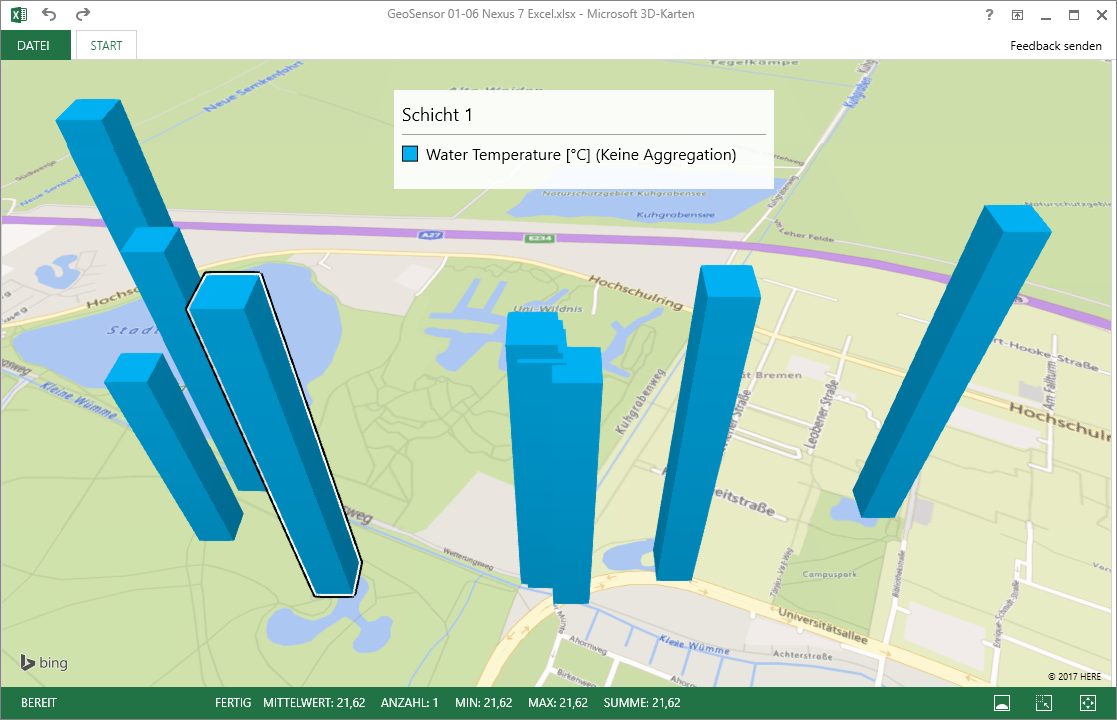
\includegraphics[width=1.0\textwidth]{src/excel_bar_graph.png}
\caption{Bar graph visualization of the field test data generated using Excel for Windows. Map data copyright 2017 HERE.}
\label{fig:excel_bar_graph}
\end{figure*}

\subsubsection{Matlab}
The version stored in Google Drive has been imported into Matlab R2017a on both the Windows 10 and the macOS 10.12 platform using a function generated by the graphical import tool and then plotted to a webmap (part of the Matlab Mapping Toolbox). The interactive webmap created by this procedure strongly resembles the map view included in the app. However, the data can then be analyzed further leveraging Matlabs manifold capabilities. A Matlab webmap generated using map data from OpenStreetMaps is shown in figure \ref{fig:matlab_webmap}. A Matlab Live Script (For Matlab R2017a including the Mapping toolbox) generating this map and the respective measure data can be found in the digital appendix.
\begin{figure*}[ht]
\centering
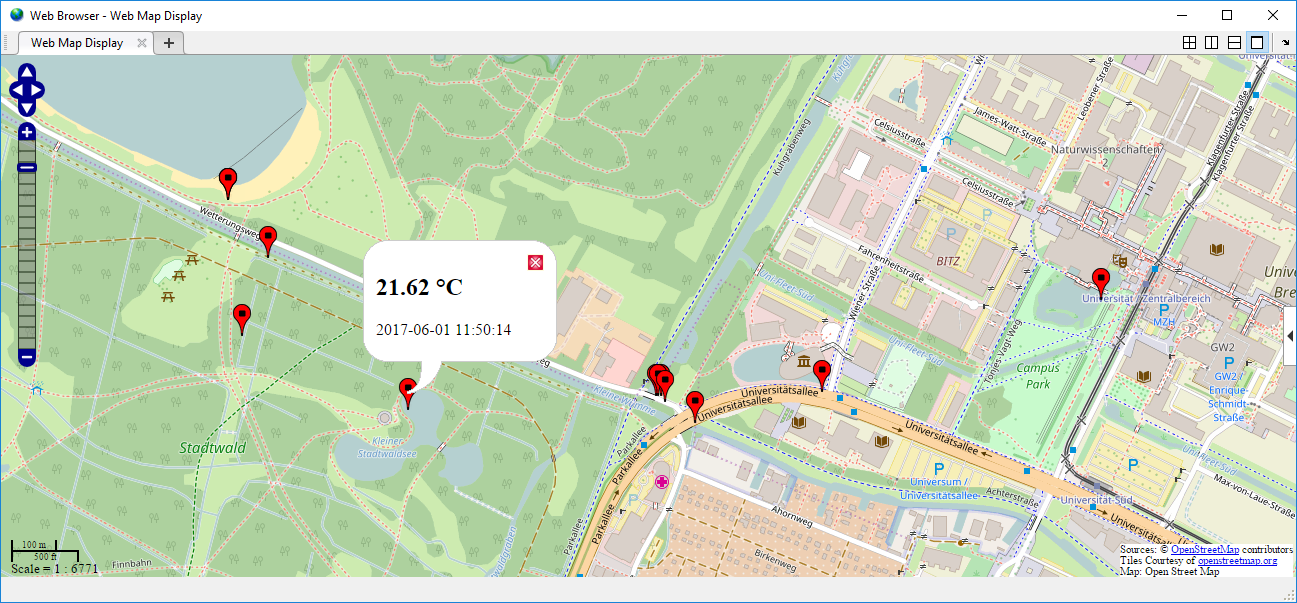
\includegraphics[width=1.0\textwidth]{src/matlab_webmap.png}
\caption{Visualisation of field test data on a Matlab webmap}
\label{fig:matlab_webmap}
\end{figure*}
\chapter{Conclusions}
In this thesis, a system for position-based data acquisition was designed. This system consists of a hardware transducer module that can easily be build based on the Arduino platform and an Android application. The hardware transducer can easily be interfaced to a multitude of sensors. In order to demonstrate the capabilities of the system a transducer device containing an air humidity, an air temperature and an encapsulated temperature sensor which might, for example, be used to measure water and soil temperatures, has been build. The system contains the capability to export data to other Android apps including cloud storage providers. 

In a system field test, the system has been proven to be able to successfully collect water and air temperature data at different waterbodies around the university of Bremen. The data from the field test has been exported to a comma separated values file which was imported and visualized in Microsoft Excel and Matlab.

A transducer device for the system can be build using an Arduino microcontroller board, a Bluetooth module, a power source and the desired sensors. The embedded software developed in this thesis is easily adaptable to use various types of sensors including but not limited to sensors providing I$^2$C, SPI, analog and UART output. When the transducer device has been built successfully, a single button press on either the transducer device or in the application user interface triggers a measurement.

As the communication protocol is fully documented, potentially a transducer device interfacing the Android app could be built from other microcontroller platforms as long as they can send correctly formatted data through a Bluetooth RFCOMM channel.

The Android application software offers a user interface following the material design introduced in Android 5.0 Lollipop but still remains compatible back to Android 2.3 Gingerbread. The software offers a visualization of the recorded data in a list and on a map (leveraging map data provided by Google maps). Data records can be deleted individually or giving a threshold for the datasets age. The data visualization can be filtered and sorted by the receive time.

Data stored in the app can be exported to a comma separated values (\texttt{.csv}) file. The decimal mark and the cell separator used in the exported file can be adjusted to suit the requirements of the software the data should be imported into. Data exported can be analyzed and visualized using most data analysis software including but not limited to Microsoft Excel and Matlab. 

\chapter{Overview of the Digital Appendix}
The digital appendix included in this thesis contains the following elements:

\begin{itemize}
\item The compiled Android application software which can be sideloaded onto compatible Android devices.
\item The source code and the build project for the Android application software. The software was developed and compiled using Android Studio.
\item The source code for the embedded software run on the Arduino in the transducer.
\item Test data recorded regarding the energy consumption and the Matlab live scripts used to generate the plots used in the thesis.
\item Test data recorded regarding the position accuracy and the Matlab live scripts used to generate the plots and maps used in the thesis.
\item Test data recorded in the field test, the Matlab live scripts used to generate the plots used in the thesis and the Excel spreadsheet used for the bar graph plot.
\item The test software used to test the protocol compliance of the Android app.
\item The fritzing (see \cite{fritzing}) files used to generate the circuit diagram and breadboard graphics.
\item The CAD files (for Autodesk Fusion 360, see \cite{f360}) used for the demonstration devices case.
\item A list of the measured properties understood and translated in the Android app.
\end{itemize}

%}}}
%{{{ Appendix

\appendix


\nocite{9783836236485}
\nocite{9783836242004}
\nocite{Ali2016}
\nocite{AndroidAPI}
\nocite{AppCompat}
\nocite{ATmega328}
\nocite{HC-05}
\nocite{JavaSpec}
\nocite{FallDetector}
\nocite{so1}
\nocite{so2}
\nocite{so3}

%}}}
%{{{ Lists

\listoffigures

% Glossary
% Der Parameter ist der Name der Datei mit den Glossareinträgen.
\cnglossary{glossary}

% Abkürzungsverzeichnis
% Der Parameter ist der Name der Datei mit der Liste der Abkürzungen.
\cnabbreviations{abbreviations}

% Literaturverzeichnis
% Nicht im Text referenzierte Dokumente zitieren, so da� sie im
% Literaturverzeichnis erscheinen


\bibliography{misc}
% Mit der Stiloption 'cnplain' erhält man Nummern 
% anstatt Namenskürzel
\bibliographystyle{plainurl}

% Stichwortverzeichnis
\cnprintindex

%}}}

\end{document}
